\documentclass[11pt]{article}
\usepackage[margin=1in]{geometry}
\usepackage{graphicx,booktabs,amsmath,hyperref,caption,float}
\usepackage[utf8]{inputenc}
\hypersetup{colorlinks=true,urlcolor=blue}
\title{The Global Renewable Electricity Transition and Its Decoupling from CO\textsubscript{2} Emissions:\\
A Reproducible Cross-Country Analysis, 2000--2022}
\author{[Author] \\ \texttt{[affiliation / email]}}
\date{This version: September 2026}

\begin{document}
\maketitle
\begin{abstract}
Between 2000 and 2022 the renewable share of global electricity rose from 18.7\% to 29.5\% of generation, yet fossil fuels still supplied roughly 61\%. This paper asks whether the electricity transition is actually loosening the link between economic growth and CO\textsubscript{2} emissions, where the effect is real, and -- crucially -- whether renewables are \emph{displacing} fossil generation or merely \emph{adding} to it. Using 163 countries over 2000--2022 (3,749 country-year observations), I combine convergence analysis, the Tapio decoupling index, and a two-way fixed-effects panel model of CO\textsubscript{2} per capita on renewable electricity share (with a lagged-renewable robustness check, a first-difference estimator, clustered standard errors, and a country-level event study). Renewable share grew fastest in countries that started lowest ($\beta=-0.024$, $p<0.001$), and the share of countries in absolute decoupling climbed from 11\% in 2000--05 to 34\% by 2017--22. Holding country and year fixed, each additional percentage point of renewable electricity is associated with about $0.61\%$ lower CO\textsubscript{2} per capita ($p<0.001$), robust to lagging, first-differencing and clustering. A second outcome -- the CO\textsubscript{2} intensity of electricity -- confirms the mechanism directly: $+1$ pp renewable share implies $2.2\%$ lower grid carbon intensity. Yet the growth is overwhelmingly \emph{additive}: globally, fossil generation rose by about 7,861 TWh over the period even as renewables rose by 5,636 TWh, and only 31\% of countries cut fossil output at all. Regional decomposition shows Europe displacing (71\% of countries cut fossil) while Africa and Asia overwhelmingly added. Under recent momentum the global renewable share reaches roughly 36\% by 2030 -- progress, but still far from displacing fossil generation.

\noindent\textbf{Keywords:} renewable electricity; decoupling; Tapio index; fixed-effects panel; carbon intensity; displacement; energy transition.
\end{abstract}

\section{Introduction}
Rising renewable electricity shares are routinely read as evidence that the energy transition is working. The harder question is whether that growth is loosening the link between economic activity and carbon emissions, and whether clean capacity is replacing dirty generation or simply riding on top of a growing system. This distinction is not semantic: it determines whether a higher renewable share is a result or merely a scoreboard.

The literature has established that high-income countries can decouple, at least relatively, and that renewable electricity helps. What remains loose is three things. First, most country-level work is descriptive -- it shows correlations without controlling for the fact that countries differ permanently in structure, climate, and industry mix. Second, it rarely asks whether the effect is uniform or concentrated in already-industrialized regions. Third, it seldom says where the current trajectory lands by 2030, the horizon most policy is actually written against. A first-difference estimator and a country-level event study around the year a country's renewable share first crosses 25\% probe whether the link is causal or merely compositional.

This study addresses those gaps with a single transparent pipeline. I document the pace and geography of the transition, test whether countries are converging, classify each country with the Tapio decoupling index across multiple windows, and then estimate the renewable--emissions relationship with a two-way fixed-effects model that holds each country's unobserved structure constant and absorbs common global shocks through year fixed effects. A lagged specification, a first-difference estimator, clustered standard errors and a second outcome (grid carbon intensity) check that the result is not an artefact of simultaneity or of mixing electricity with other sectors. A constant-momentum projection closes with 2030.

\section{Literature review and conceptual framework}
The relationship between economic growth and environmental pressure has been framed since the 1990s by the Environmental Kuznets Curve (EKC) hypothesis and, more usefully for policy, by the concept of \emph{decoupling}. The OECD (2002) defines decoupling as a decline in the ratio of environmental pressure to economic activity, distinguishing \emph{relative} decoupling (the ratio falls while pressure still rises) from \emph{absolute} decoupling (pressure falls outright). Tapio (2005) operationalized this for transport with an elasticity index that separates the two and has since been applied to energy--CO\textsubscript{2} systems.

Applied work has reached two broad conclusions. The first is that absolute decoupling of CO\textsubscript{2} from GDP is achievable but rare and geographically concentrated: Steinberger and Roberts (2010) and Jackson and Papathanasopoulou (2008) show it almost exclusively in mature, post-industrial economies, while much of the Global South remains coupled or expansively coupled. The second is that renewable electricity is the leading lever. Semieniuk et al. (2021) and the IPCC (2022) argue that low-carbon electricity deployment is the single largest contributor to modelled emission reductions, and the IEA (2023) attributes the majority of recent power-sector emission declines to renewables and nuclear.

Two gaps motivate this paper. First, the decoupling and renewable-deployment literatures are rarely joined in a single identification design that controls for permanent country differences; pooled correlations can be driven by unobserved structural factors that fixed effects absorb. Second, and more important, the literature tends to equate a rising renewable \emph{share} with falling fossil \emph{generation}. They are not the same. A renewable build that rides on top of a growing system can raise the share while fossil output keeps climbing -- what I call the \emph{addition} case, as opposed to genuine \emph{displacement}. Hickel and Kallis (2020) and the broader green-growth debate stress exactly this point: without absolute reductions in fossil throughput, a higher clean share is a scoreboard, not a result. This paper measures both the decoupling link and the displacement mechanism, and shows they can point in different directions.

\section{Data and methods}
Data come from Our World in Data's energy and CO\textsubscript{2} datasets (CC-BY), merged at the country-year level. I keep sovereign countries (OWID aggregates and ``World'' removed), years 2000--2022, and require non-missing renewable share, fossil share, low-carbon share, CO\textsubscript{2}, GDP, population and electricity generation. This yields 163 countries and 3,749 country-year observations. Shares are generation-weighted at the global and regional level so that large producers count proportionally. Summary statistics appear in Table~\ref{tab:desc}.

Five methods follow.
\paragraph{Convergence.} $\beta$-convergence regresses each country's annual log growth in renewable share on its initial log level; a negative slope means laggards grew faster. $\sigma$-convergence tracks the cross-country standard deviation of the share over time.
\paragraph{Decoupling.} The Tapio index divides the growth rate of CO\textsubscript{2} by the growth rate of GDP over a window; values below zero are absolute decoupling, $0$--$0.8$ relative, $0.8$--$1.2$ coupling, above $1.2$ expansive coupling.
\paragraph{The core estimate.} A panel model of $\ln(\text{CO}_2\text{ per capita})$ on renewable electricity share, $\ln(\text{GDP per capita})$, country fixed effects and year fixed effects. Standard errors are reported two ways -- heteroskedasticity-robust (HC1) and clustered by country -- and an $F$-test confirms the country fixed effects are jointly significant (rejecting pooled OLS).
\paragraph{A second outcome.} Because CO\textsubscript{2} per capita mixes electricity with all other sectors, I also estimate $\ln(\text{CO}_2\ \text{intensity of electricity},\ \text{gCO}_2/\text{kWh})$ on renewable share with the same fixed-effects structure; a fall in grid carbon intensity is the most direct evidence that renewables replace fossil plant.
\paragraph{Identification deepening.} A one-year lag of renewable share, a first-difference estimator, and a country-level event study around the 25\% renewable threshold probe the direction and stability of the link.

\begin{table}[H]
\centering
\caption{Descriptive statistics, country-year observations, 2000--2022.}
\label{tab:desc}
\begin{tabular}{lcccc}
\toprule
Variable & Mean & SD & Min & Max \\
\midrule
Renewables share of electricity (\%) & 34.51 & 33.45 & 0.00 & 100.00 \\
Fossil share of electricity (\%) & 60.71 & 34.08 & 0.00 & 100.00 \\
Low-carbon share of electricity (\%) & 39.29 & 34.08 & 0.00 & 100.00 \\
CO\textsubscript{2} per capita (t) & 4.92 & 6.56 & 0.02 & 67.73 \\
GDP per capita (intl \$) & 16,270 & 18,071 & 422 & 163,531 \\
Electricity demand per capita (kWh) & 3,862 & 5,594 & 9 & 56,049 \\
CO\textsubscript{2} intensity of electricity (gCO\textsubscript{2}/kWh) & 447.5 & 253.9 & 0.0 & 1,306.7 \\
\bottomrule
\end{tabular}
\end{table}

\section{Results}

\subsection{The pace and geography of the transition}
Globally, renewables rose from 18.7\% of generation in 2000 to 29.5\% in 2022, a gain of 10.7 percentage points. The rate is not constant: the compound annual growth was 2.1\% over the full period but 3.6\% from 2015 onward, an acceleration that lines up with the post-Paris deployment push. Fossil fuels, by contrast, barely moved -- from 64.6\% to 61.4\% ($-3.2$ points). The geography is uneven: Oceania, the Americas and Europe lead, while Asia sits lowest despite being the manufacturing core.

\begin{figure}[H]
\centering
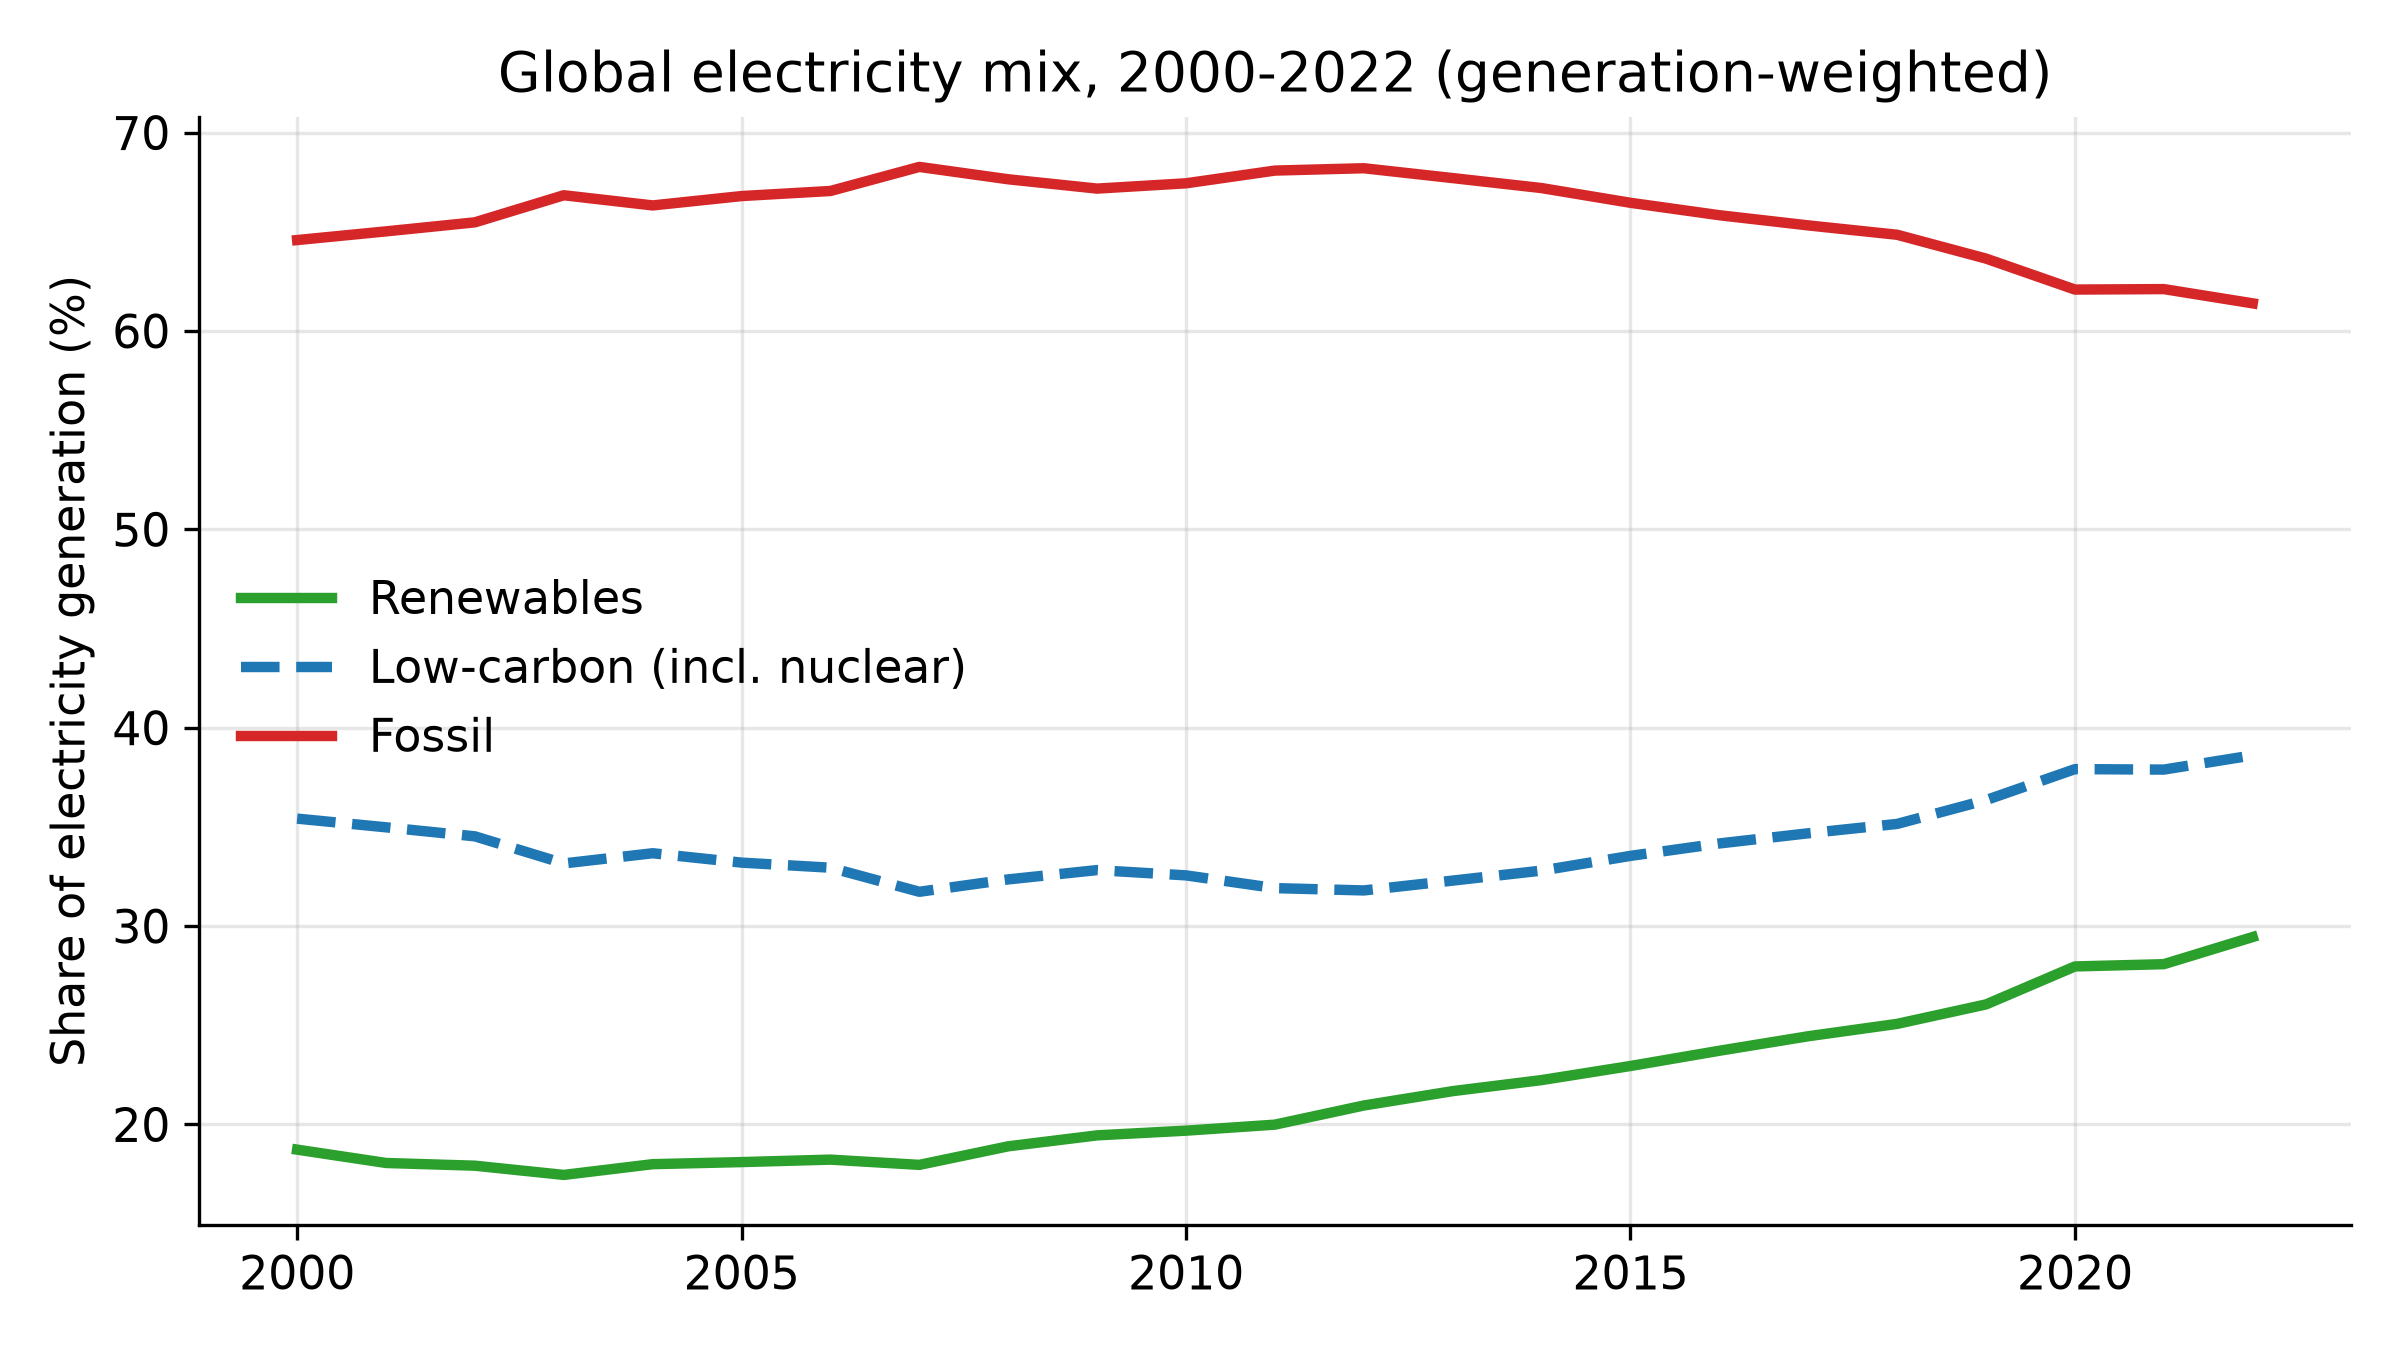
\includegraphics[width=0.85\textwidth]{figures/figure1_global_trend.png}
\caption{Generation-weighted global electricity mix, 2000--2022. Renewables climb steadily; fossil stays dominant.}
\end{figure}

\begin{figure}[H]
\centering
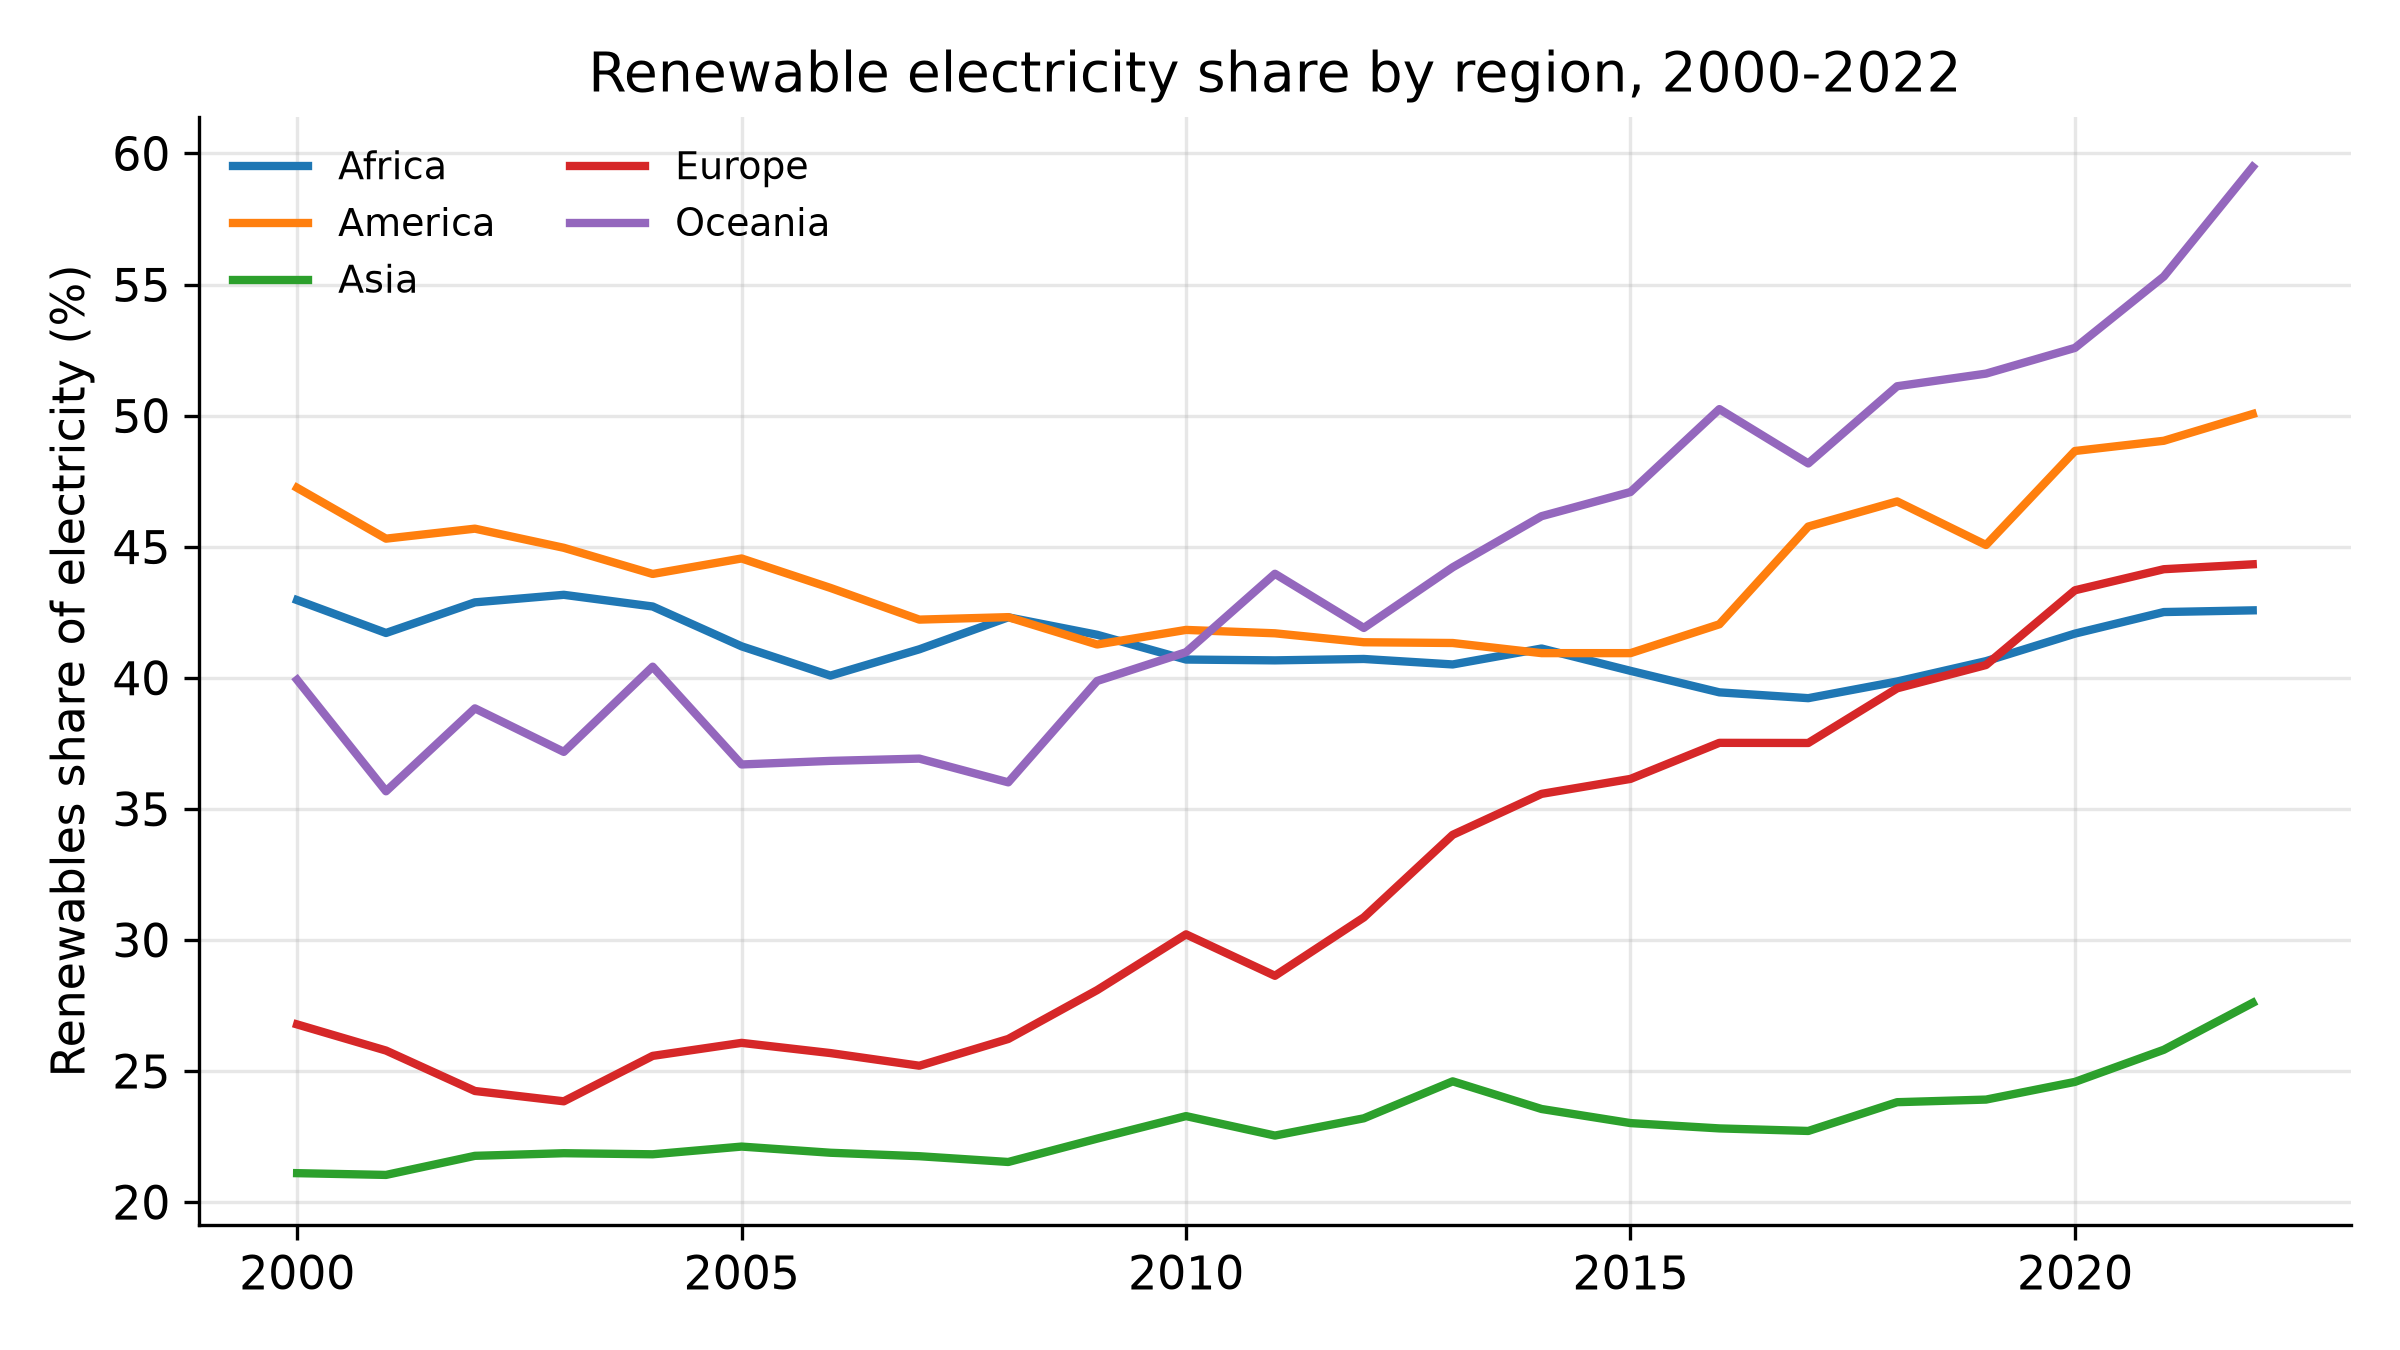
\includegraphics[width=0.8\textwidth]{figures/figure2_regional.png}
\caption{Renewable electricity share by region, 2022. Asia sits lowest despite being the manufacturing core; Oceania, the Americas and Europe lead.}
\end{figure}

\subsection{Convergence: the laggards are catching up}
The $\beta$-convergence slope is $-0.024$ (SE 0.0019, $p<0.001$, $R^2=0.55$), meaning countries with the lowest initial renewable share grew fastest. The cross-country dispersion also narrowed: the standard deviation of renewable share fell from 35.1 to 32.5 points ($-7.6$\%).

\begin{figure}[H]
\centering
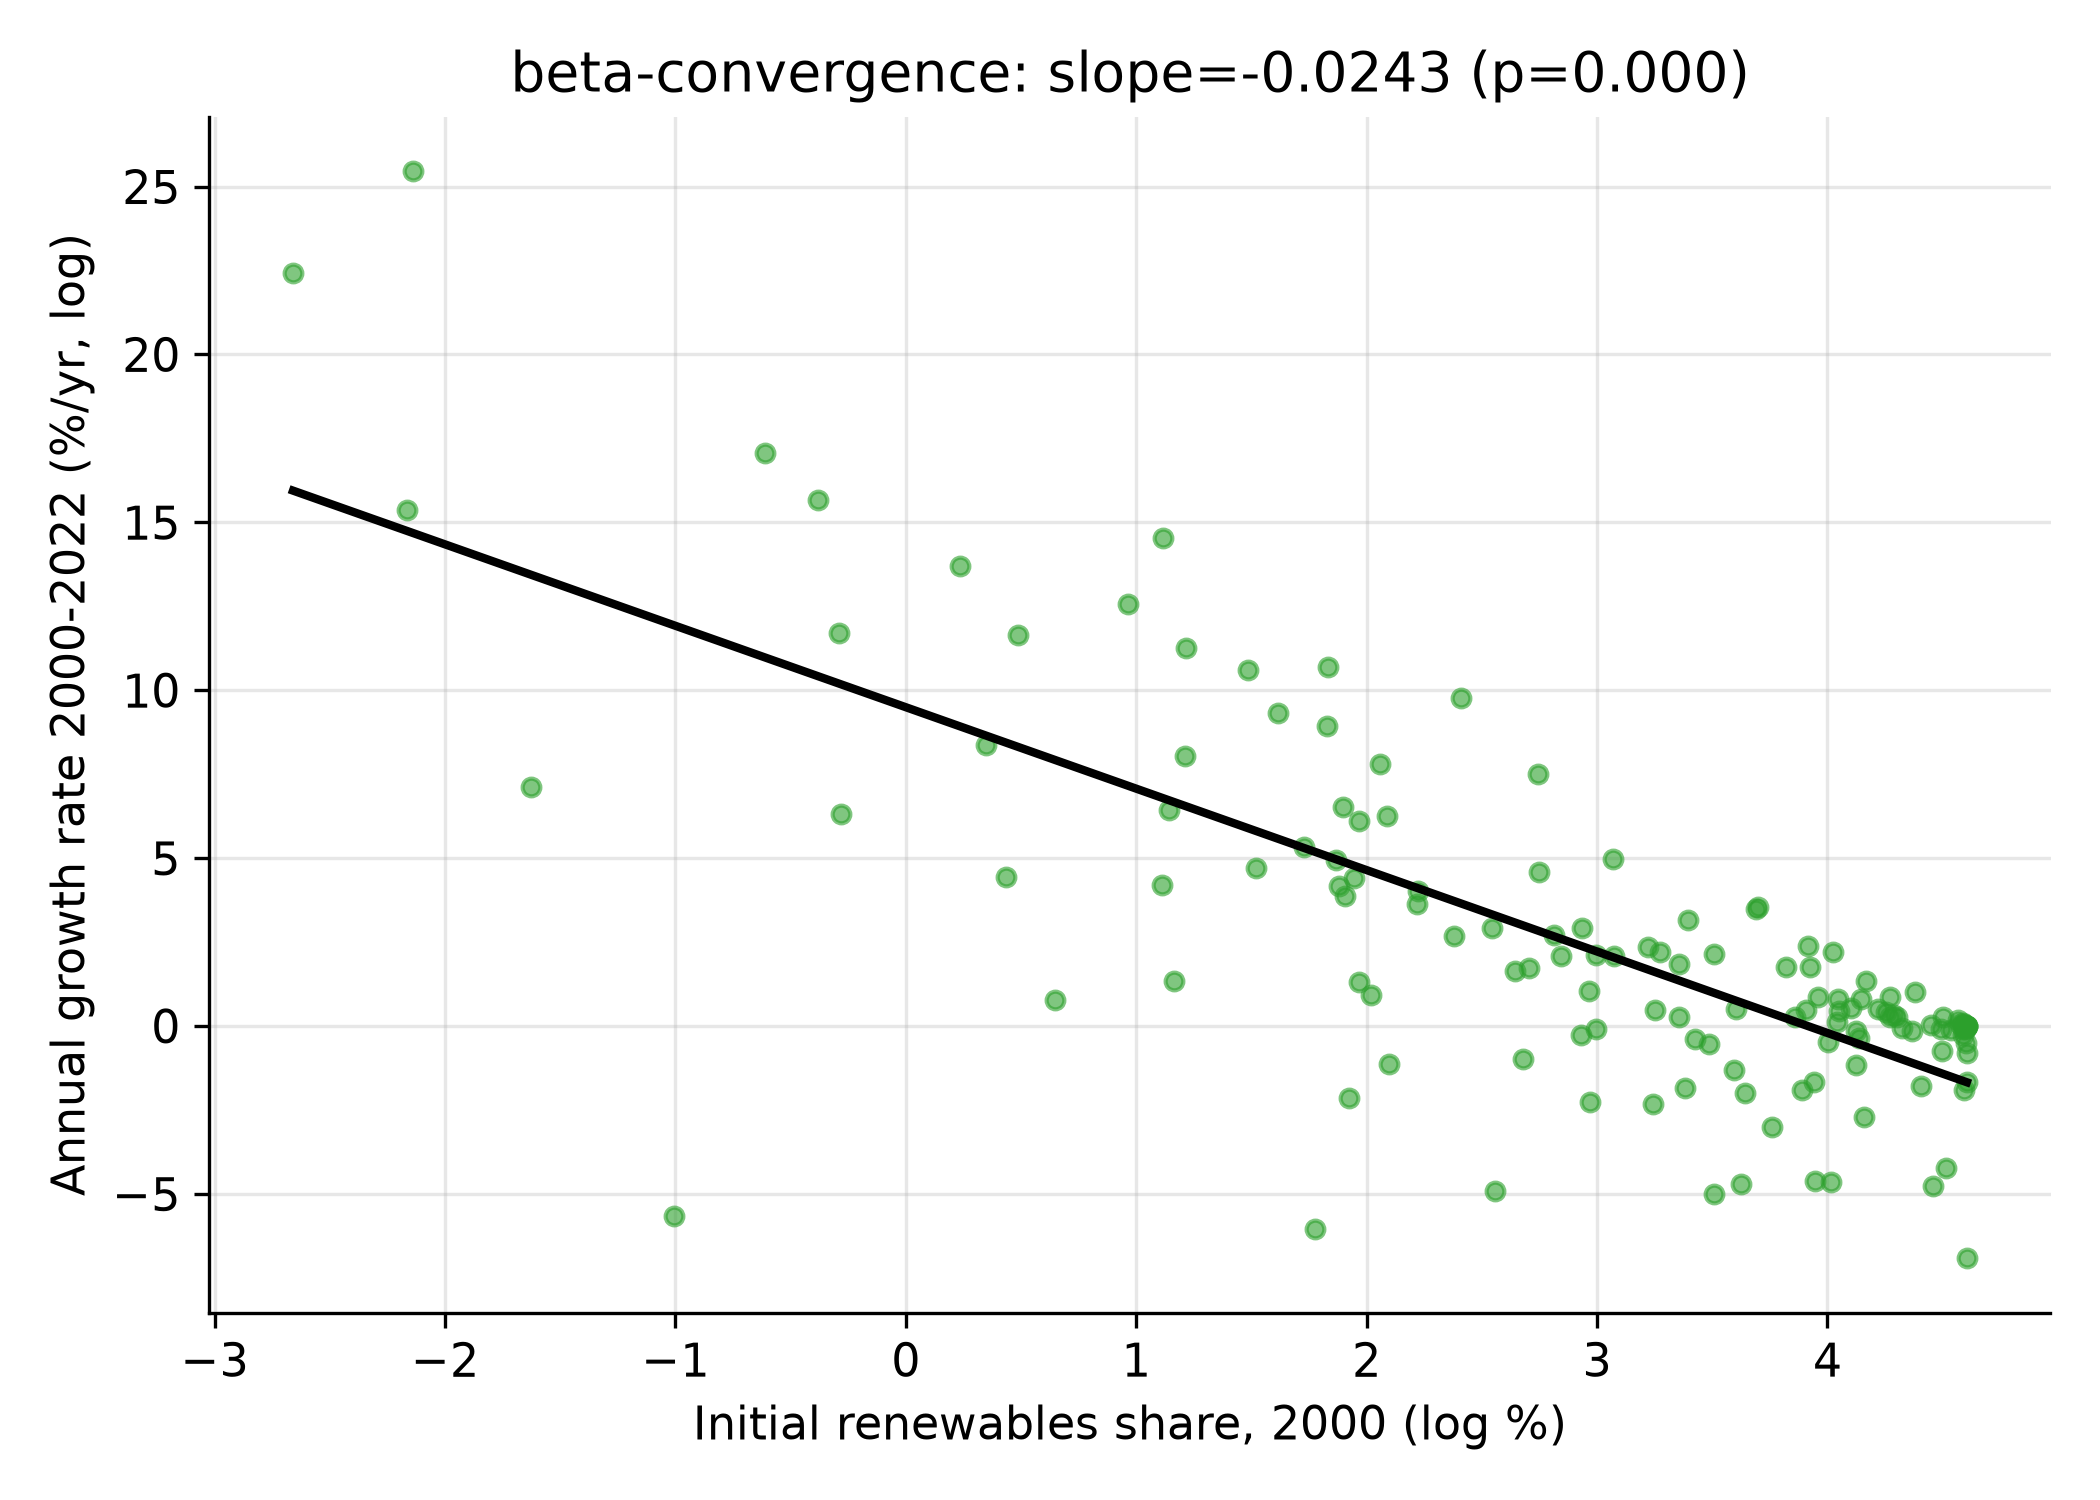
\includegraphics[width=0.8\textwidth]{figures/figure3_beta.png}
\caption{$\beta$-convergence in renewable electricity share. A downward slope means countries that started lower grew faster.}
\end{figure}

\subsection{Decoupling: more countries are breaking the link}
Across 163 countries, 25.8\% achieved absolute decoupling (CO\textsubscript{2} fell while GDP rose), 38.7\% relative decoupling, and 31.9\% stayed coupled or worse. The average decoupling index was 0.63, and the correlation between renewable gain and the decoupling index was $-0.22$. The share of countries in absolute decoupling rose from 11.0\% in 2000--05 to 33.7\% in 2017--22.

\begin{figure}[H]
\centering
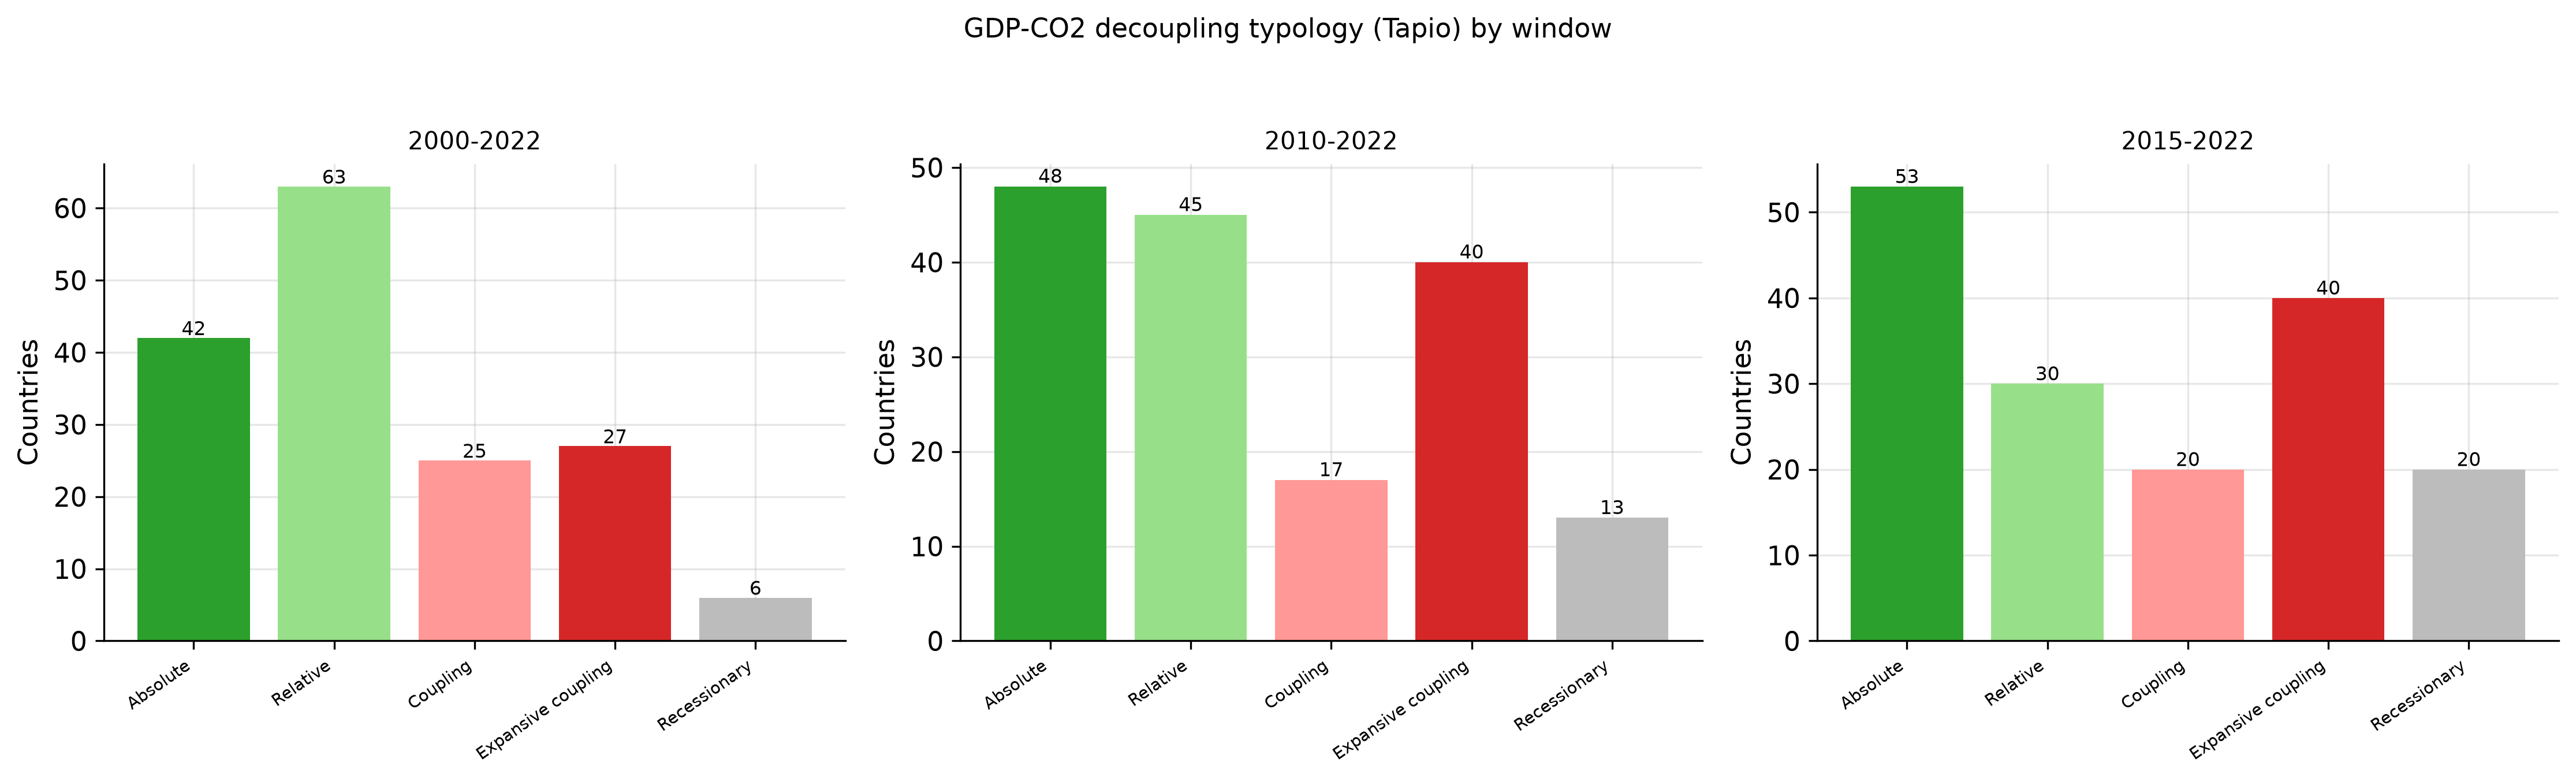
\includegraphics[width=0.8\textwidth]{figures/figure4_tapio.png}
\caption{Tapio decoupling typology across three windows. Absolute decoupling (green) expands in later windows.}
\end{figure}

\begin{figure}[H]
\centering
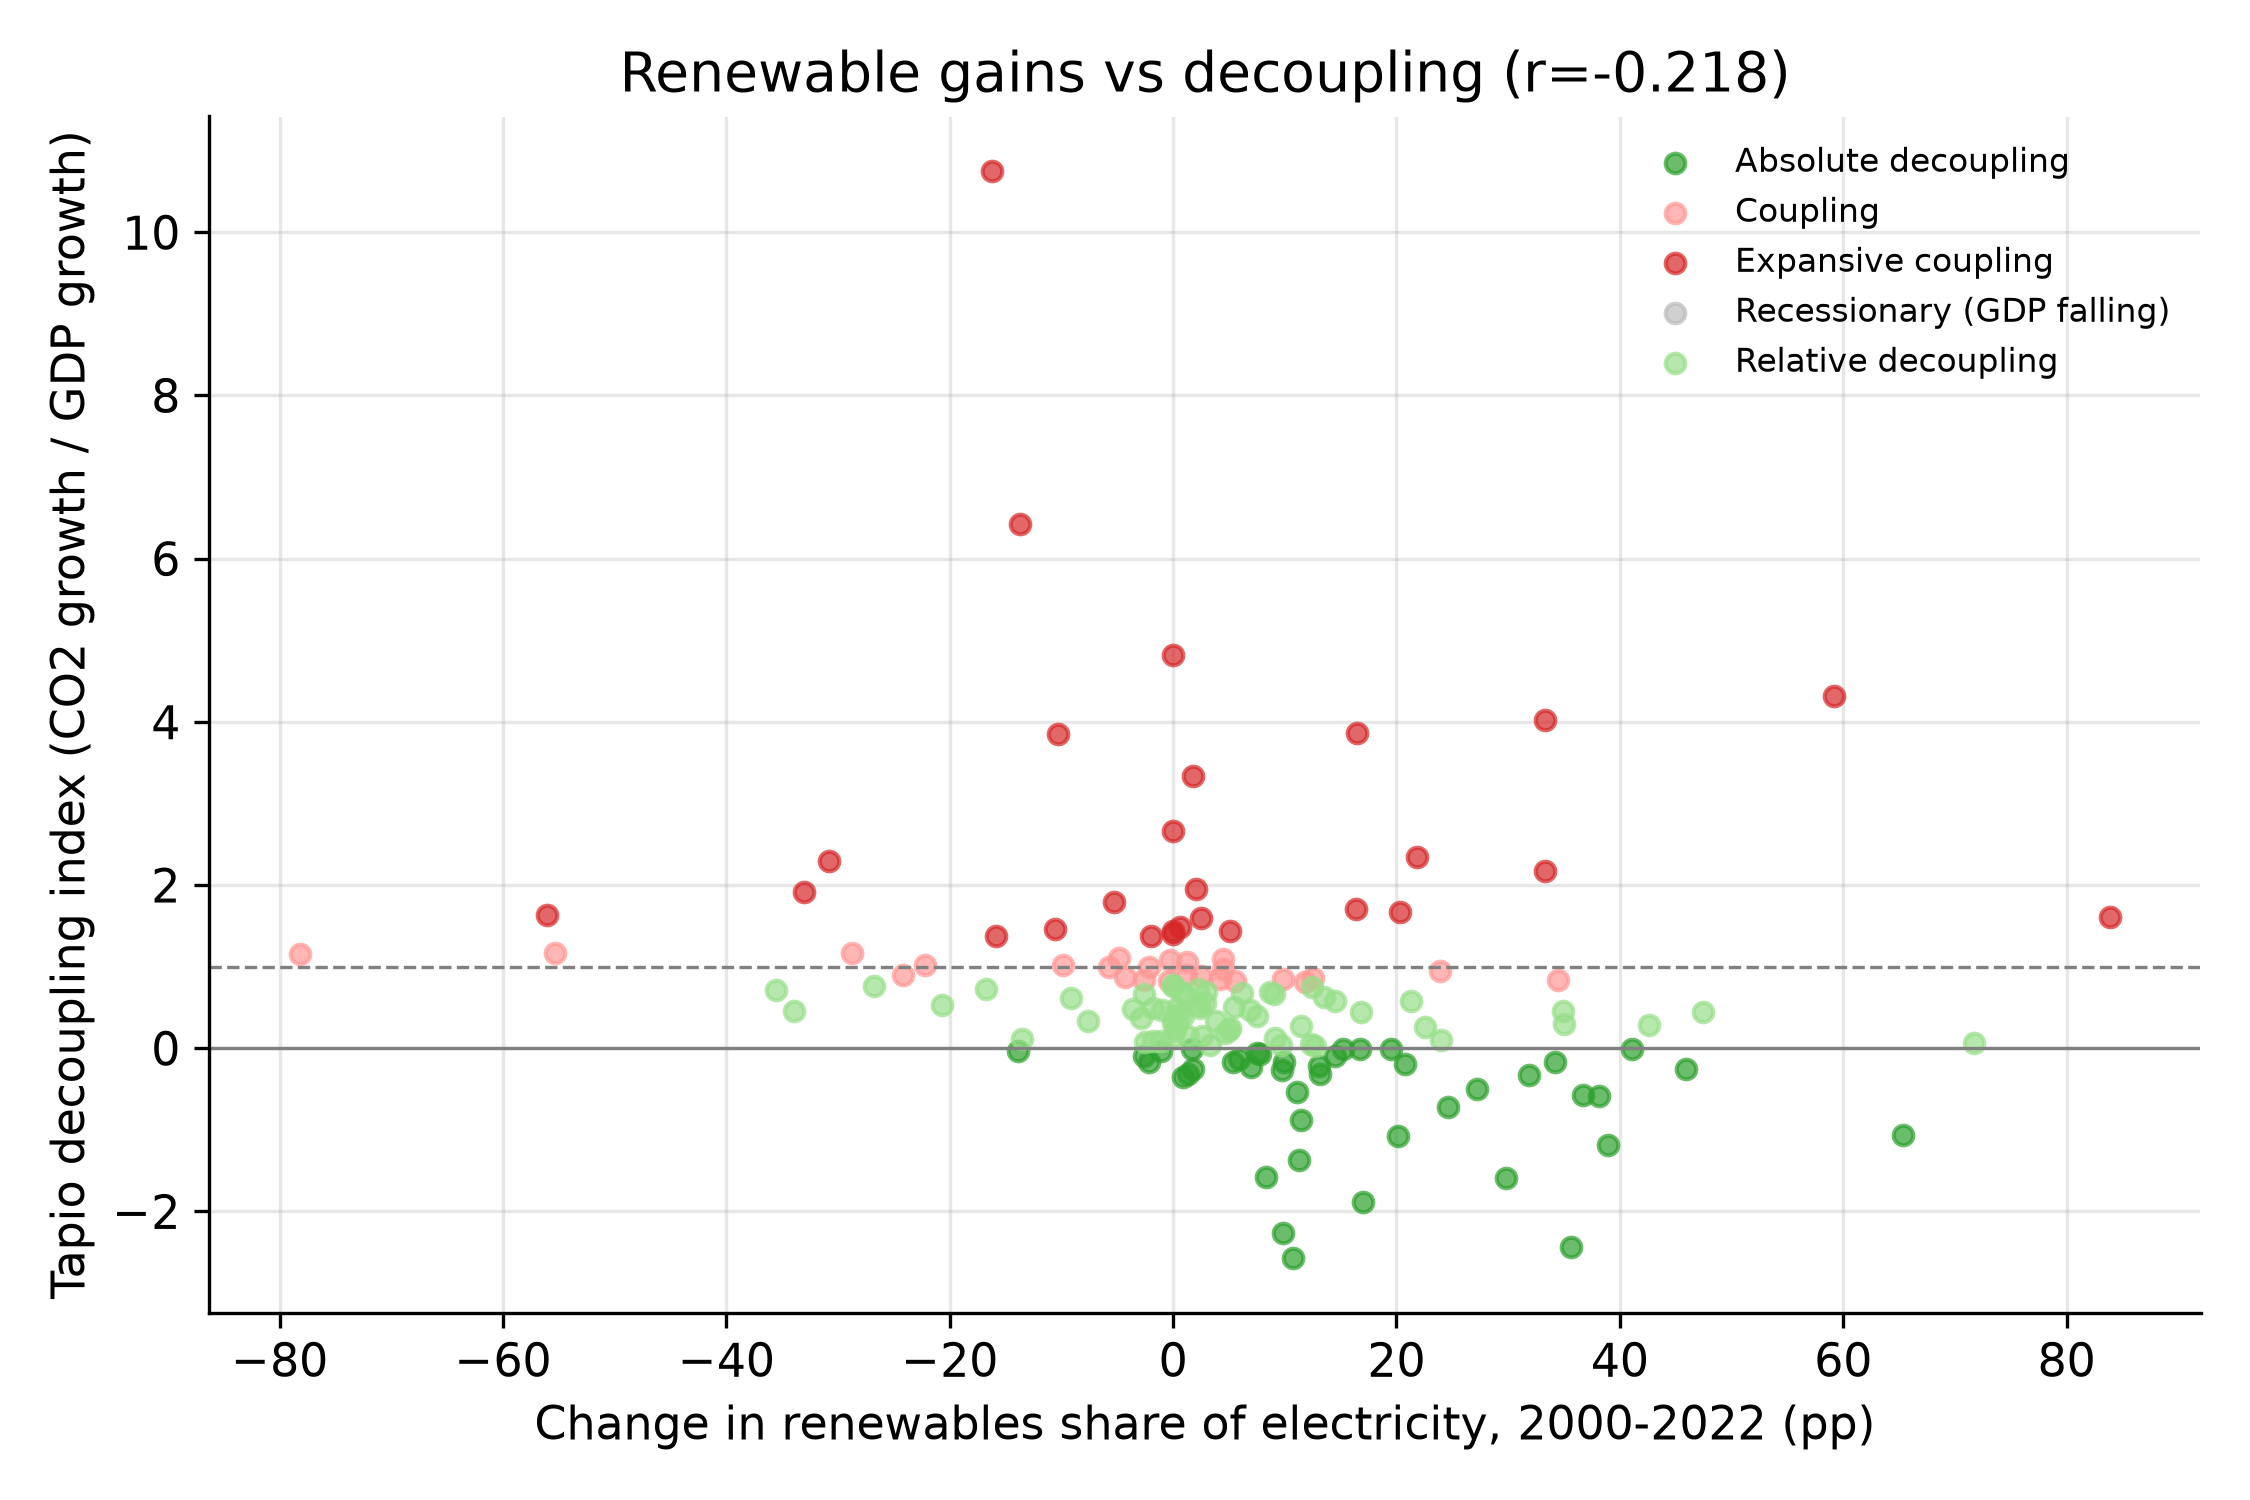
\includegraphics[width=0.8\textwidth]{figures/figure5_renew_decoupling.png}
\caption{Renewable-share gain versus the Tapio decoupling index. Countries below zero (absolute decoupling) cluster at higher renewable gains.}
\end{figure}

\begin{figure}[H]
\centering
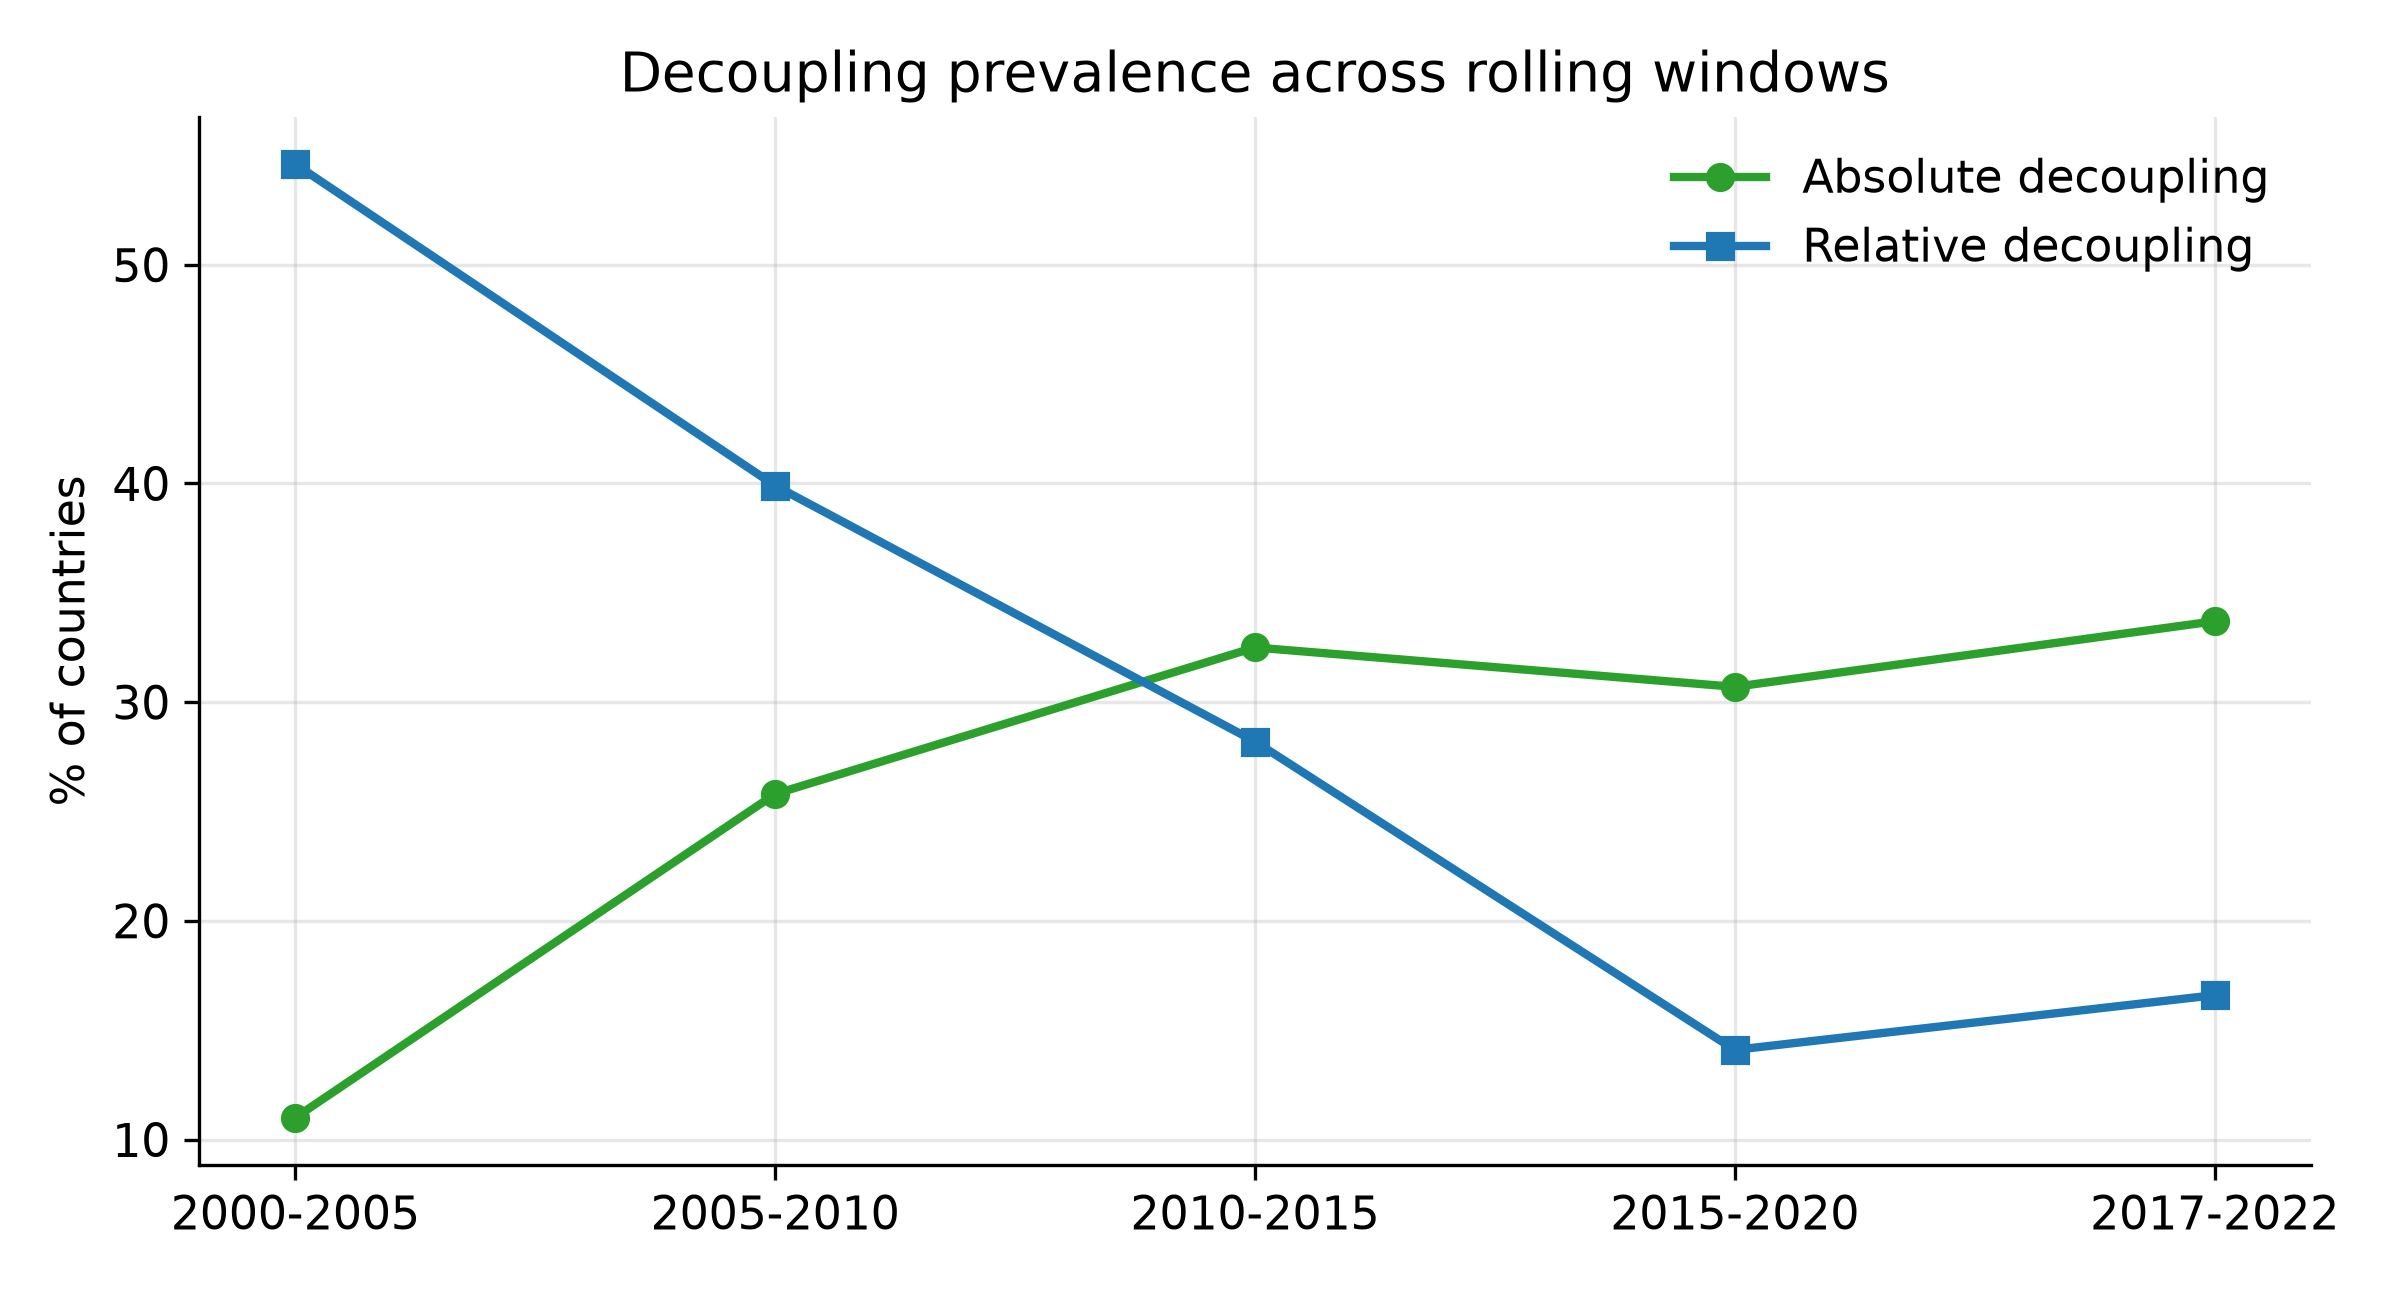
\includegraphics[width=0.8\textwidth]{figures/figure6_prevalence.png}
\caption{Prevalence of absolute and relative decoupling across rolling windows. Absolute decoupling (green) widens over time.}
\end{figure}

\subsection{The renewable--emissions link, held to account}
The fixed-effects model controls for permanent country structure. Table~\ref{tab:fe} reports a sequence of specifications. The baseline -- country and year fixed effects -- gives a coefficient of $-0.0061$ on renewable share (about $0.61\%$ lower CO\textsubscript{2} per capita per $+1$ pp, $p<0.001$). The magnitude is stable as we add a demand control, lag the renewable variable, and move to a first-difference estimator. Country fixed effects are jointly highly significant ($F=148.1$, $p<0.001$), justifying the fixed-effects specification over pooled OLS. Standard errors are essentially unchanged when clustered by country (SE $=0.002$).

\begin{table}[H]
\centering
\caption{Renewable electricity share and $\ln(\text{CO}_2\text{ per capita})$, two-way fixed effects. Dependent variable is $\ln(\text{CO}_2\text{ pc})$ in specs 1--5 and the year-on-year change in $\ln(\text{CO}_2\text{ pc})$ in spec 6. Coefficient is the change per $+1$ pp renewable share. *** $p<0.01$.}
\label{tab:fe}
\begin{tabular}{lcccc}
\toprule
Specification & Coef & SE (HC1) & SE (cluster) & N \\
\midrule
1. Pooled OLS & $-0.00773^{***}$ & 0.00028 & 0.00121 & 3,749 \\
2. Country FE & $-0.00605^{***}$ & 0.00056 & 0.00194 & 3,749 \\
3. Country + Year FE (baseline) & $-0.00607^{***}$ & 0.00057 & 0.00200 & 3,749 \\
4. + Demand control & $-0.00472^{***}$ & 0.00049 & 0.00153 & 3,749 \\
5. Lagged renewable & $-0.00513^{***}$ & 0.00059 & 0.00198 & 3,586 \\
6. First-difference & $-0.00650^{***}$ & 0.00148 & 0.00095 & 121 \\
\bottomrule
\end{tabular}
\end{table}

The link is not uniform across space (Figure~\ref{fig:het}). It is large and highly significant in Europe ($-0.53$/pp, $p<0.001$) and the Americas ($-0.76$/pp, $p<0.001$). In Asia the point estimate is negative but not significant at conventional levels ($-0.19$/pp, $p=0.46$), and in Africa it is small and only marginally significant ($-0.12$/pp, $p=0.085$). This is the regional mirror of the tercile result below: the clearest emissions dividend appears where renewable penetration is already substantial, and it is least certain in the still-expanding Asian and African systems -- the very regions where Section~4.7 shows renewables being added on top of, rather than displacing, fossil generation.

\begin{table}[H]
\centering
\caption{Heterogeneity of the renewable--emissions effect by region (country + year fixed effects; \% change in CO\textsubscript{2}/capita per $+1$ pp renewable share, 95\% CI).}
\label{tab:het}
\begin{tabular}{lcccc}
\toprule
Region & Coef (\%/pp) & SE & $p$ & $N$ \\
\midrule
Americas & $-0.76$ & 0.05 & $<0.001$ & 621 \\
Europe & $-0.53$ & 0.07 & $<0.001$ & 874 \\
Asia & $-0.19$ & 0.26 & 0.46 & 1,058 \\
Africa & $-0.12$ & 0.07 & 0.085 & 1,150 \\
\bottomrule
\end{tabular}
\end{table}

The effect is also heterogeneous through time, not only across space. Splitting countries into terciles by their 2000 renewable share, the emissions-reducing coefficient is strongest exactly where renewable penetration was already high: in the top tercile (2000 share $>48.8$\%) each $+1$ pp cuts CO\textsubscript{2}/capita by about $0.66\%$ ($p<0.001$), in the middle tercile $0.45$/pp ($p<0.001$), but in the bottom tercile (2000 share $\le 6.5$\%) the coefficient is small and not significant ($-0.23$/pp, $p=0.15$). Renewables deliver the clearest emissions dividend where the grid is already largely clean and marginal capacity displaces the remaining fossil; the dividend has not yet materialised in the still-expanding low-baseline systems.

\begin{figure}[H]
\centering
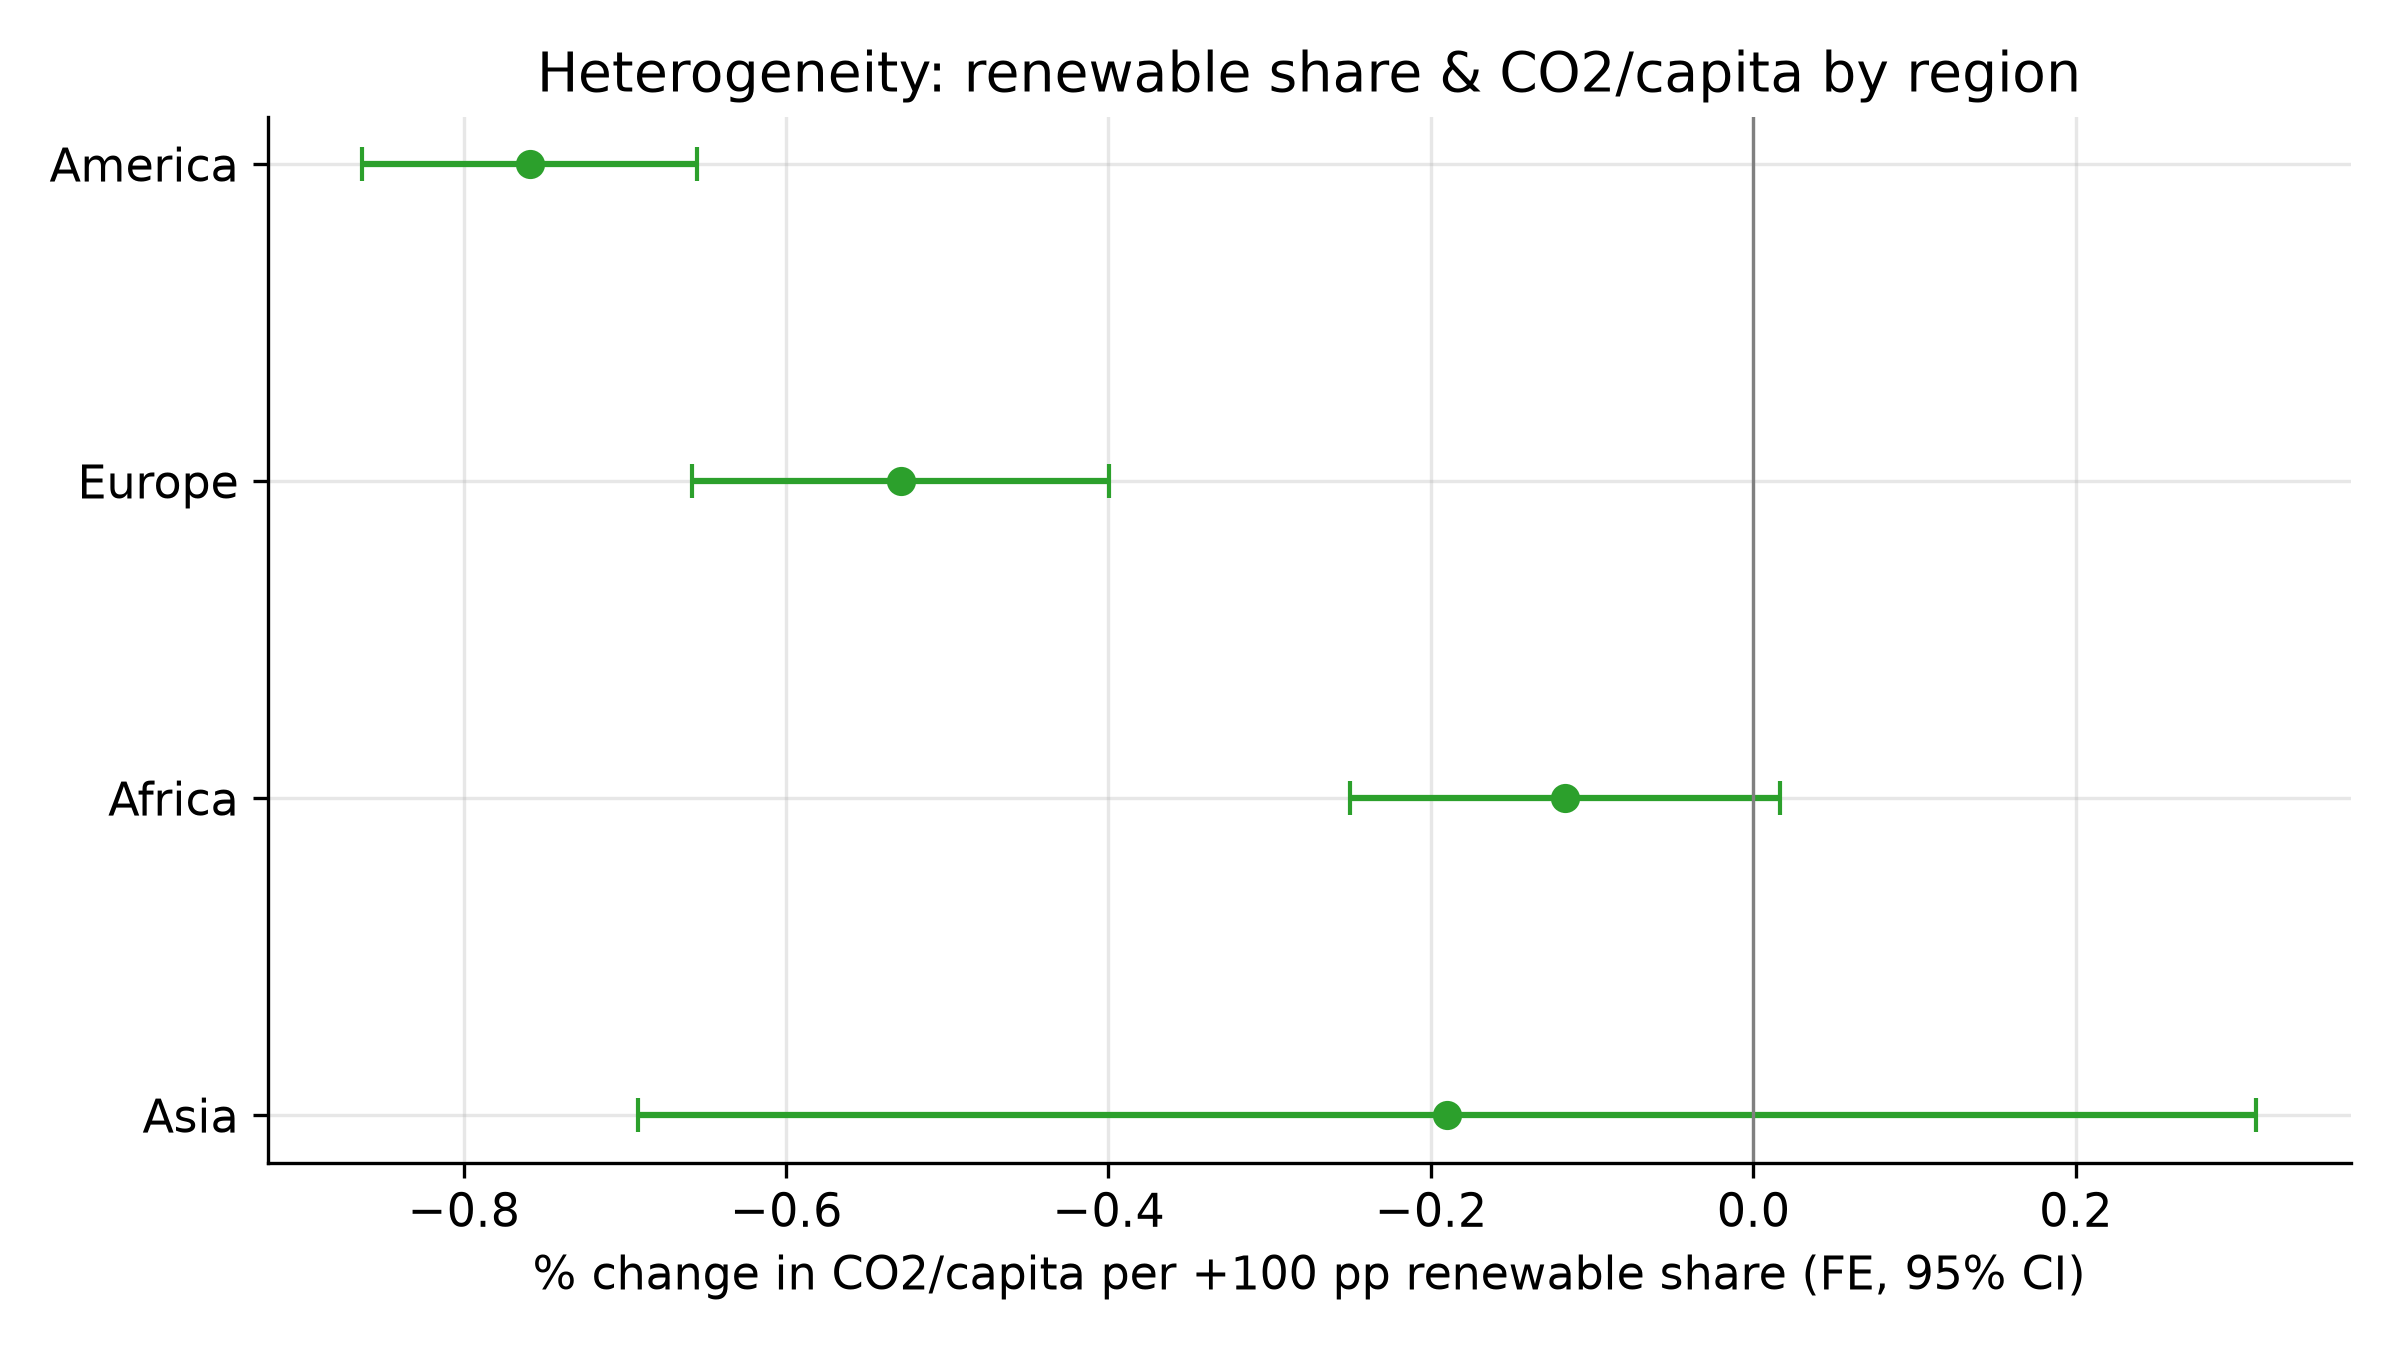
\includegraphics[width=0.8\textwidth]{figures/figure7_heterogeneity.png}
\caption{Regional fixed-effects estimates (\% change in CO\textsubscript{2}/capita per +100 pp renewable share, 95\% CI). Africa's interval includes zero.}
\end{figure}

\begin{table}[H]
\centering
\caption{Heterogeneity by 2000 renewable-share tercile (country + year fixed effects; \% change in CO\textsubscript{2}/capita per $+1$ pp renewable share, 95\% CI).}
\label{tab:terc}
\begin{tabular}{lcccc}
\toprule
Tercile (2000 renewable share) & Coef (\%/pp) & SE & $p$ & $N$ \\
\midrule
Low ($\le 6.5\%$) & $-0.23$ & 0.16 & 0.15 & 1,265 \\
Mid ($6.5$--$48.8\%$) & $-0.45$ & 0.08 & $<0.001$ & 1,242 \\
High ($>48.8\%$) & $-0.66$ & 0.08 & $<0.001$ & 1,242 \\
\bottomrule
\end{tabular}
\end{table}

\subsection{A cleaner test: the carbon intensity of electricity}
CO\textsubscript{2} per capita conflates power with every other emitting sector. To test displacement more directly, I re-estimate the same fixed-effects model with the dependent variable as the CO\textsubscript{2} intensity of electricity (gCO\textsubscript{2}/kWh). A one-percentage-point rise in renewable share is associated with $2.2\%$ lower grid carbon intensity (coef $-0.0222$, SE 0.00085, clustered SE 0.00291, $p<0.001$, $N=3,728$, $R^2=0.97$). Average grid intensity also falls monotonically across deciles of renewable share (Figure~\ref{fig:ci}). This confirms the decoupling link is not an artefact of GDP or population -- it shows up in the physics of the grid itself.

\begin{figure}[H]
\centering
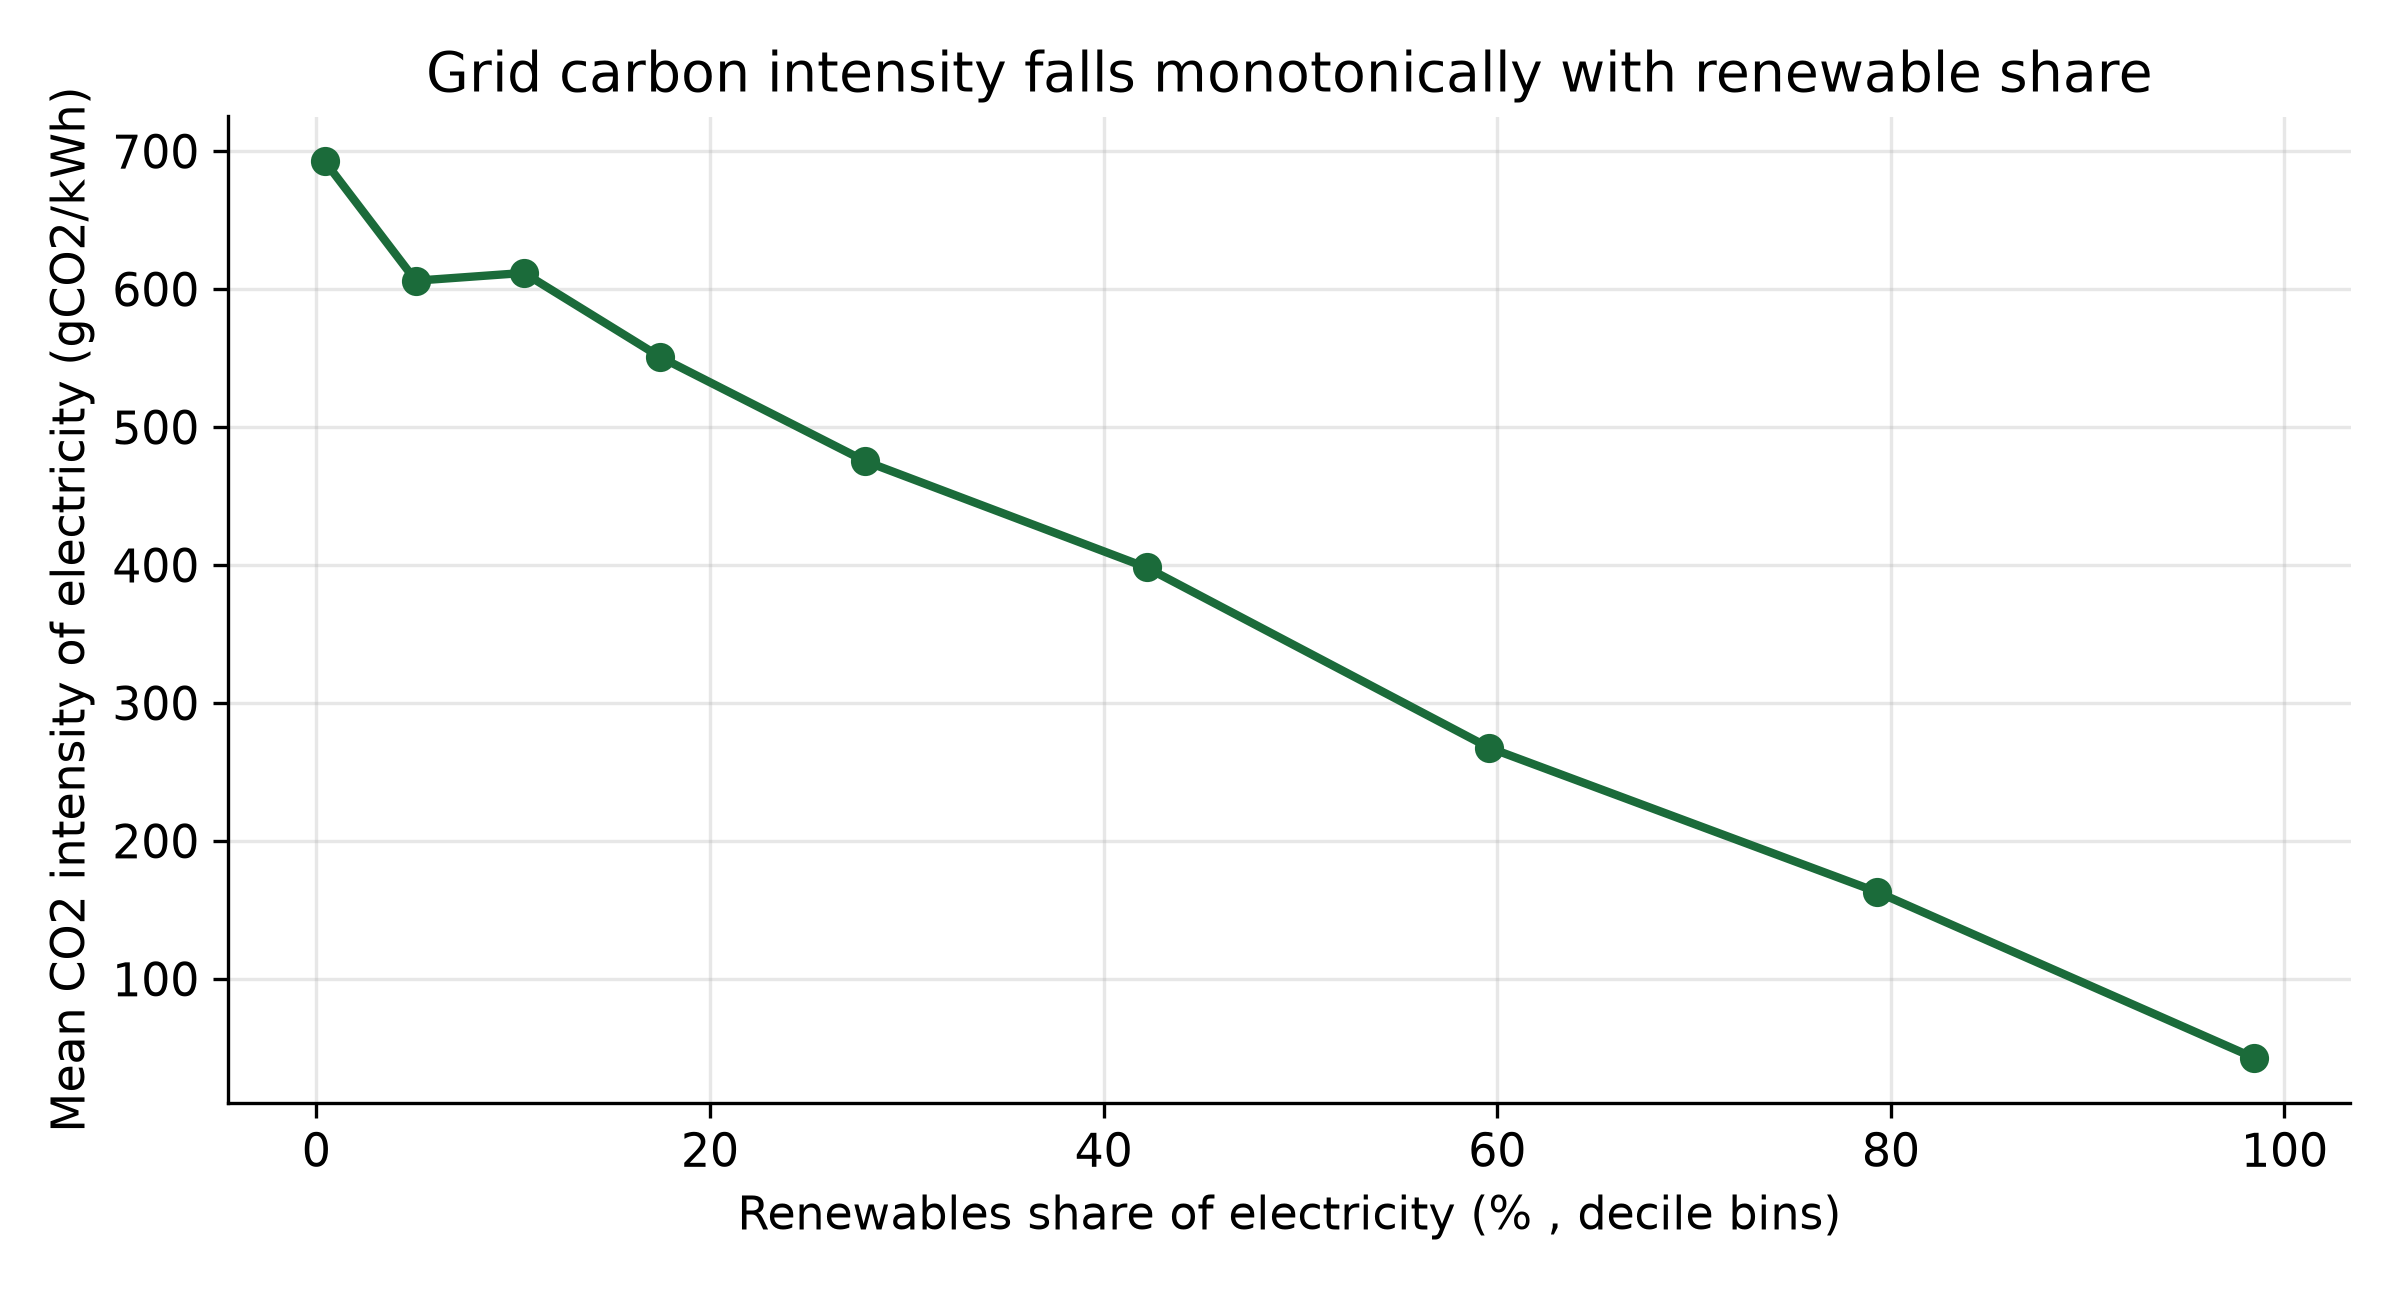
\includegraphics[width=0.8\textwidth]{figures/figure12_carbon_intensity.png}
\caption{Mean CO\textsubscript{2} intensity of electricity by decile of renewable share. Grids get cleaner as renewables rise.}
\label{fig:ci}
\end{figure}

\subsection{Identification: an event study and a within-country check}
The first-difference estimator (spec 6) removes every factor fixed within a country; a one-point year-on-year rise in renewable share is associated with about $0.65\%$ lower CO\textsubscript{2} per capita in the same step ($p<0.001$). The event study traces emissions around each country's first crossing of 25\% renewable share (20 countries with sufficient pre/post data). Emissions were already drifting down before the event and continued -- and slightly steepened -- afterward, with no discrete break (post-event average deviation $-10.8\%$, $p=0.058$). Decarbonization in this sample is a momentum process, not a switch that flips at a round-number threshold.

\begin{figure}[H]
\centering
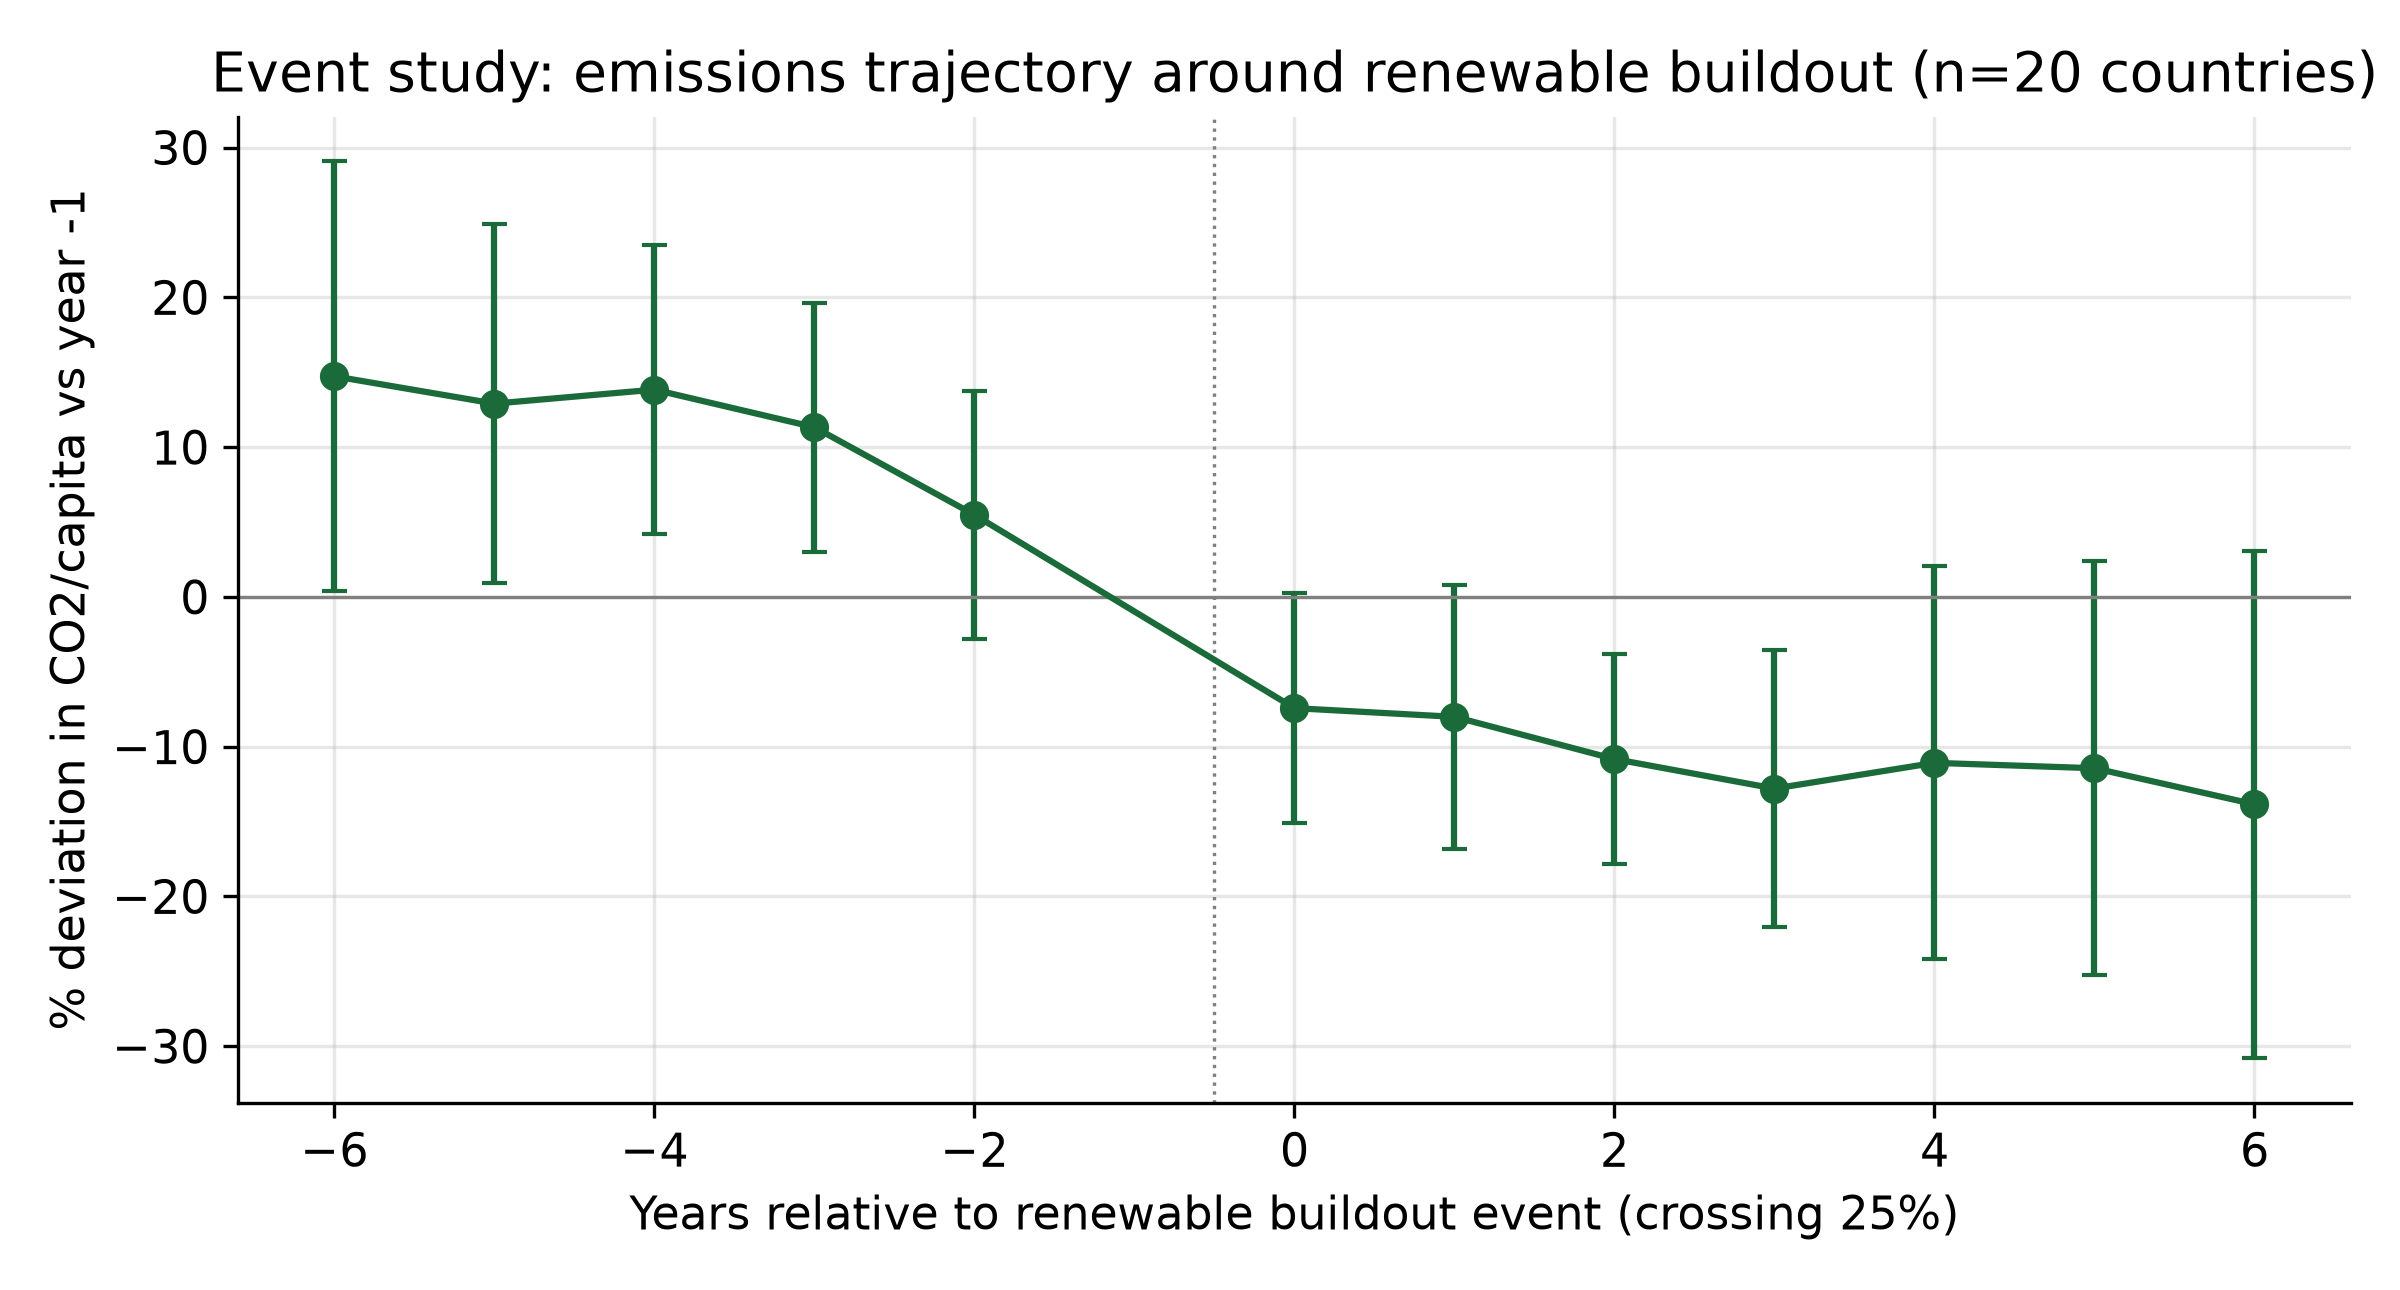
\includegraphics[width=0.8\textwidth]{figures/figure9_event_study.png}
\caption{Event study around the year a country's renewable share first crosses 25\%. Coefficients are \% deviation of CO\textsubscript{2}/capita from the year before the event.}
\end{figure}

\subsection{Mechanism: displacing, or just adding?}
The fixed-effects and event-study results say renewables go with lower emissions per capita. They do not say renewables are replacing fossil. Between 2000 and 2022 the world added 5,636 TWh of renewables and 7,861 TWh of fossil generation. Fossil output grew by roughly 1.4 times as much as renewables in absolute terms; total generation nearly doubled, from 15,225 to 28,820 TWh. The displacement ratio is $-1.40$ (negative = additive). Only 51 of 163 countries (31\%) actually cut their fossil generation, and the correlation between renewable-share gain and change in fossil generation is essentially zero (0.00).

The regional decomposition makes the mechanism explicit (Figure~\ref{fig:dispreg}). Europe is the only major region where renewables \emph{displaced} fossil: its displacement ratio is positive ($+0.34$) and 71\% of European countries cut fossil generation. By contrast, Africa ($-2.54$, 16\% displacing) and Asia ($-2.29$, 13\% displacing) added fossil far faster than renewables. The renewable--emissions coefficient is therefore not a universal law; it is the statistical signature of regions that happened to retire carbon as they built clean.

\begin{figure}[H]
\centering
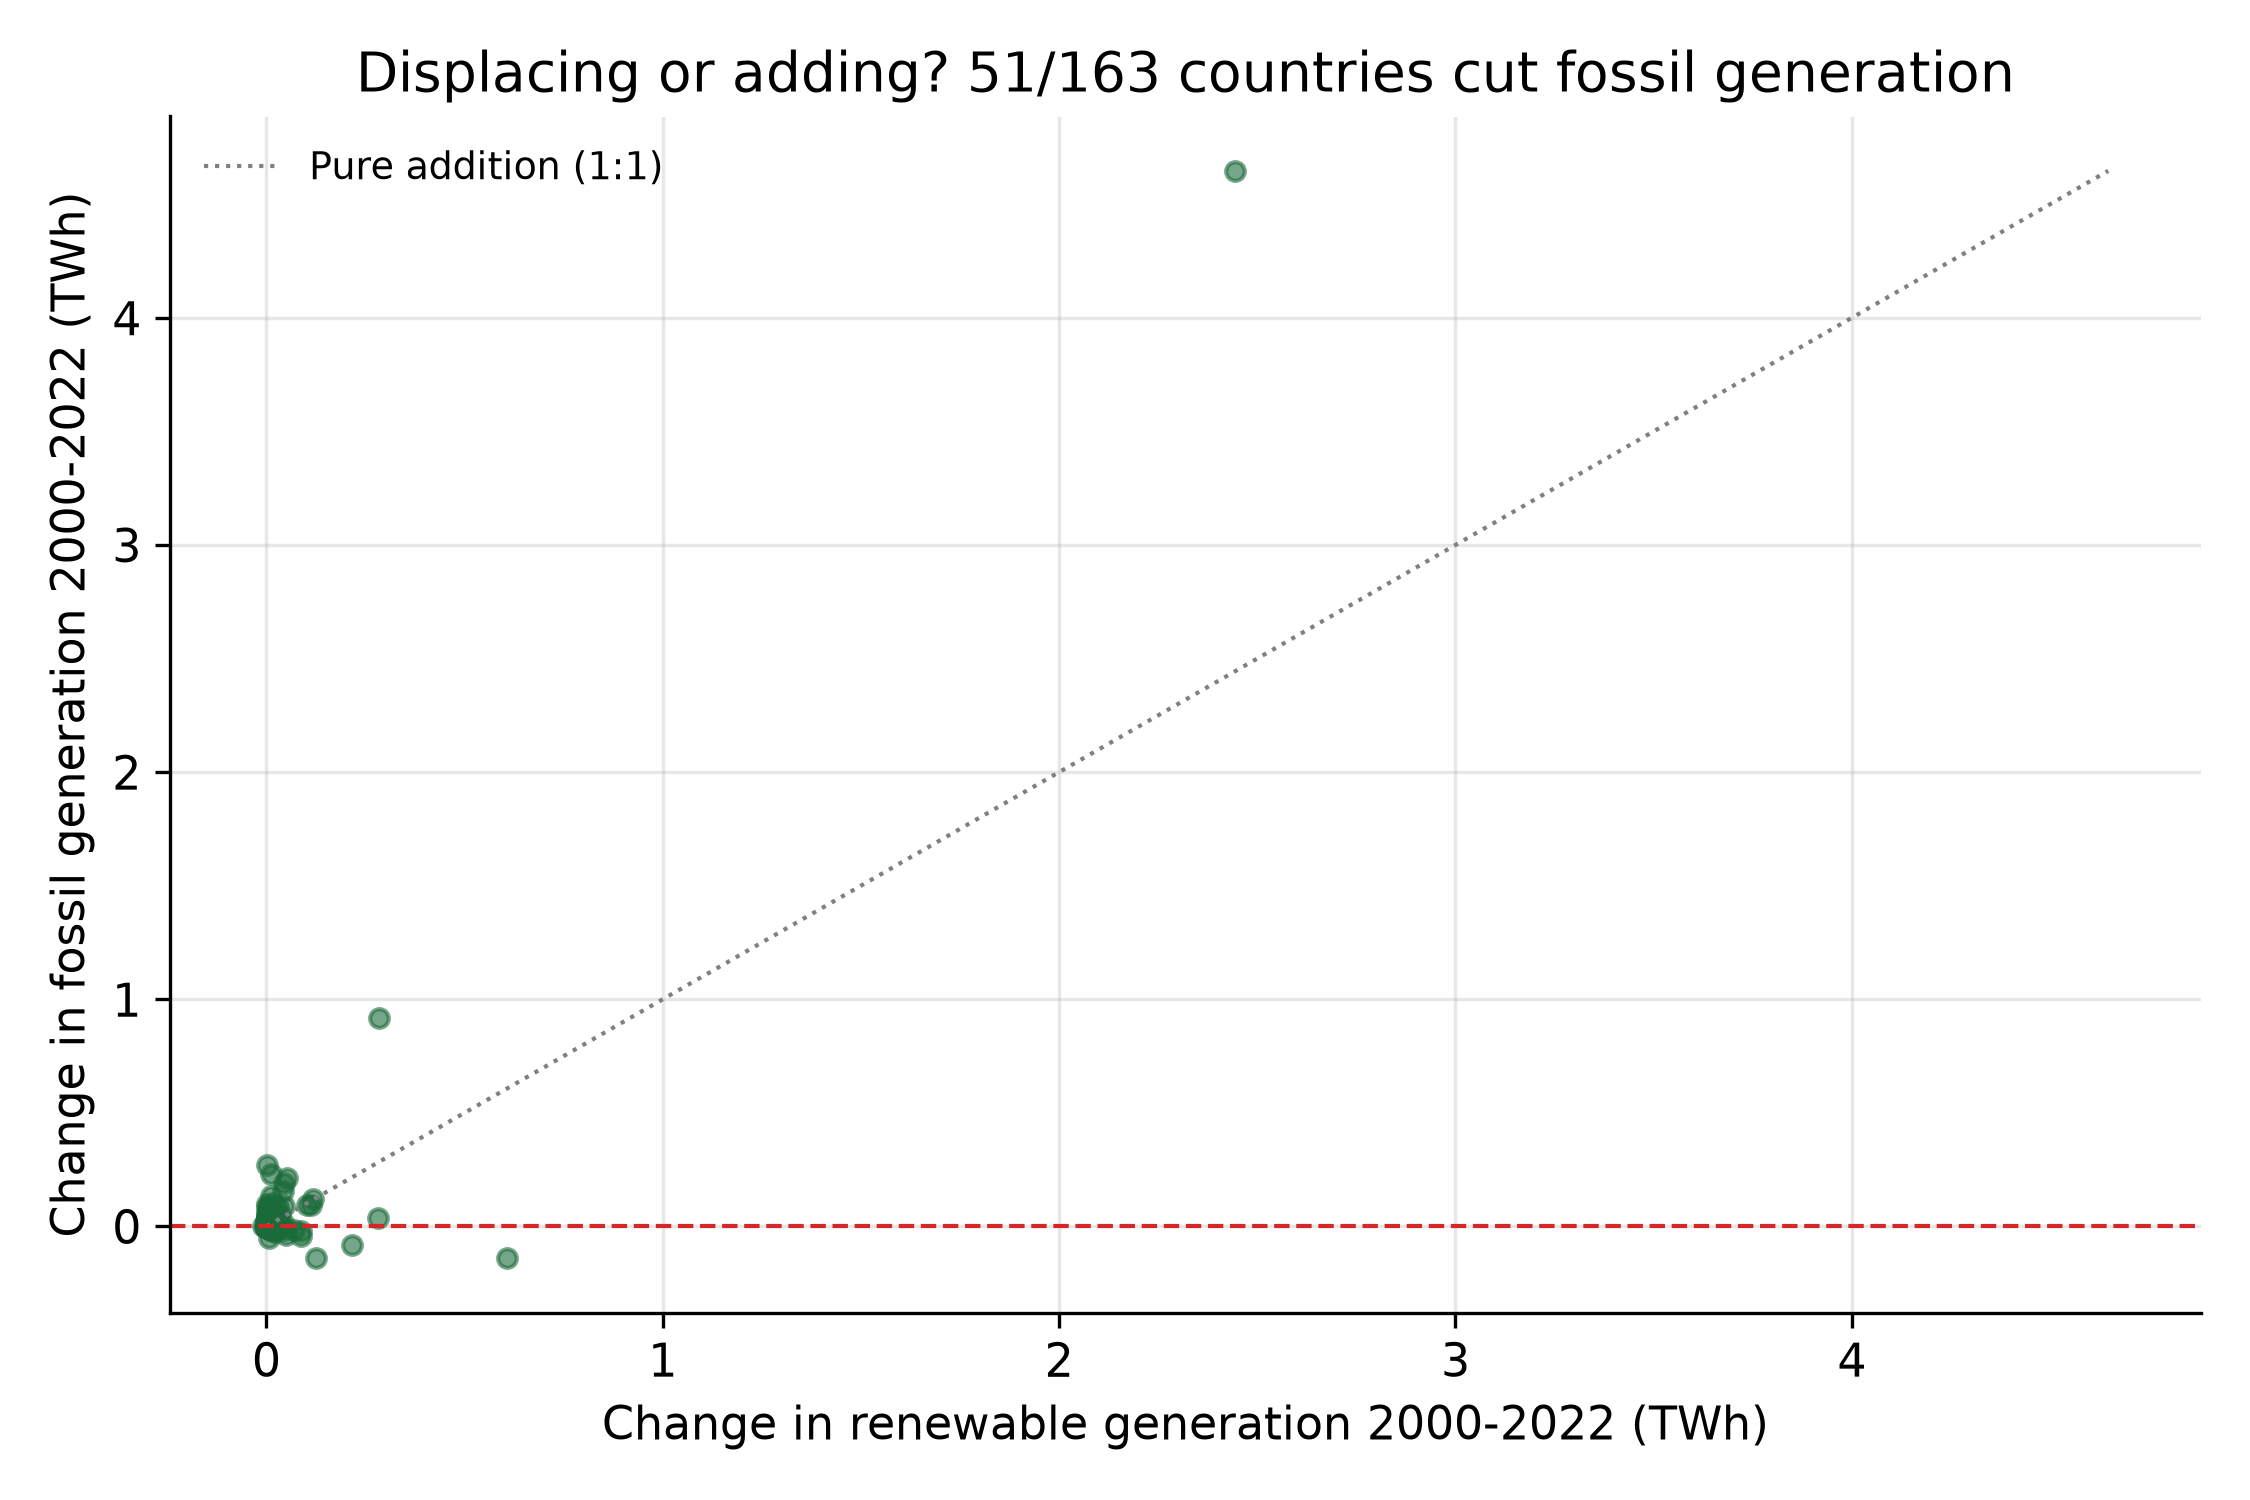
\includegraphics[width=0.8\textwidth]{figures/figure10_displacement.png}
\caption{Change in fossil vs renewable generation, 2000--2022, per country. Most points sit above zero: fossil generation rose. Only 31\% of countries cut fossil output.}
\end{figure}

\begin{figure}[H]
\centering
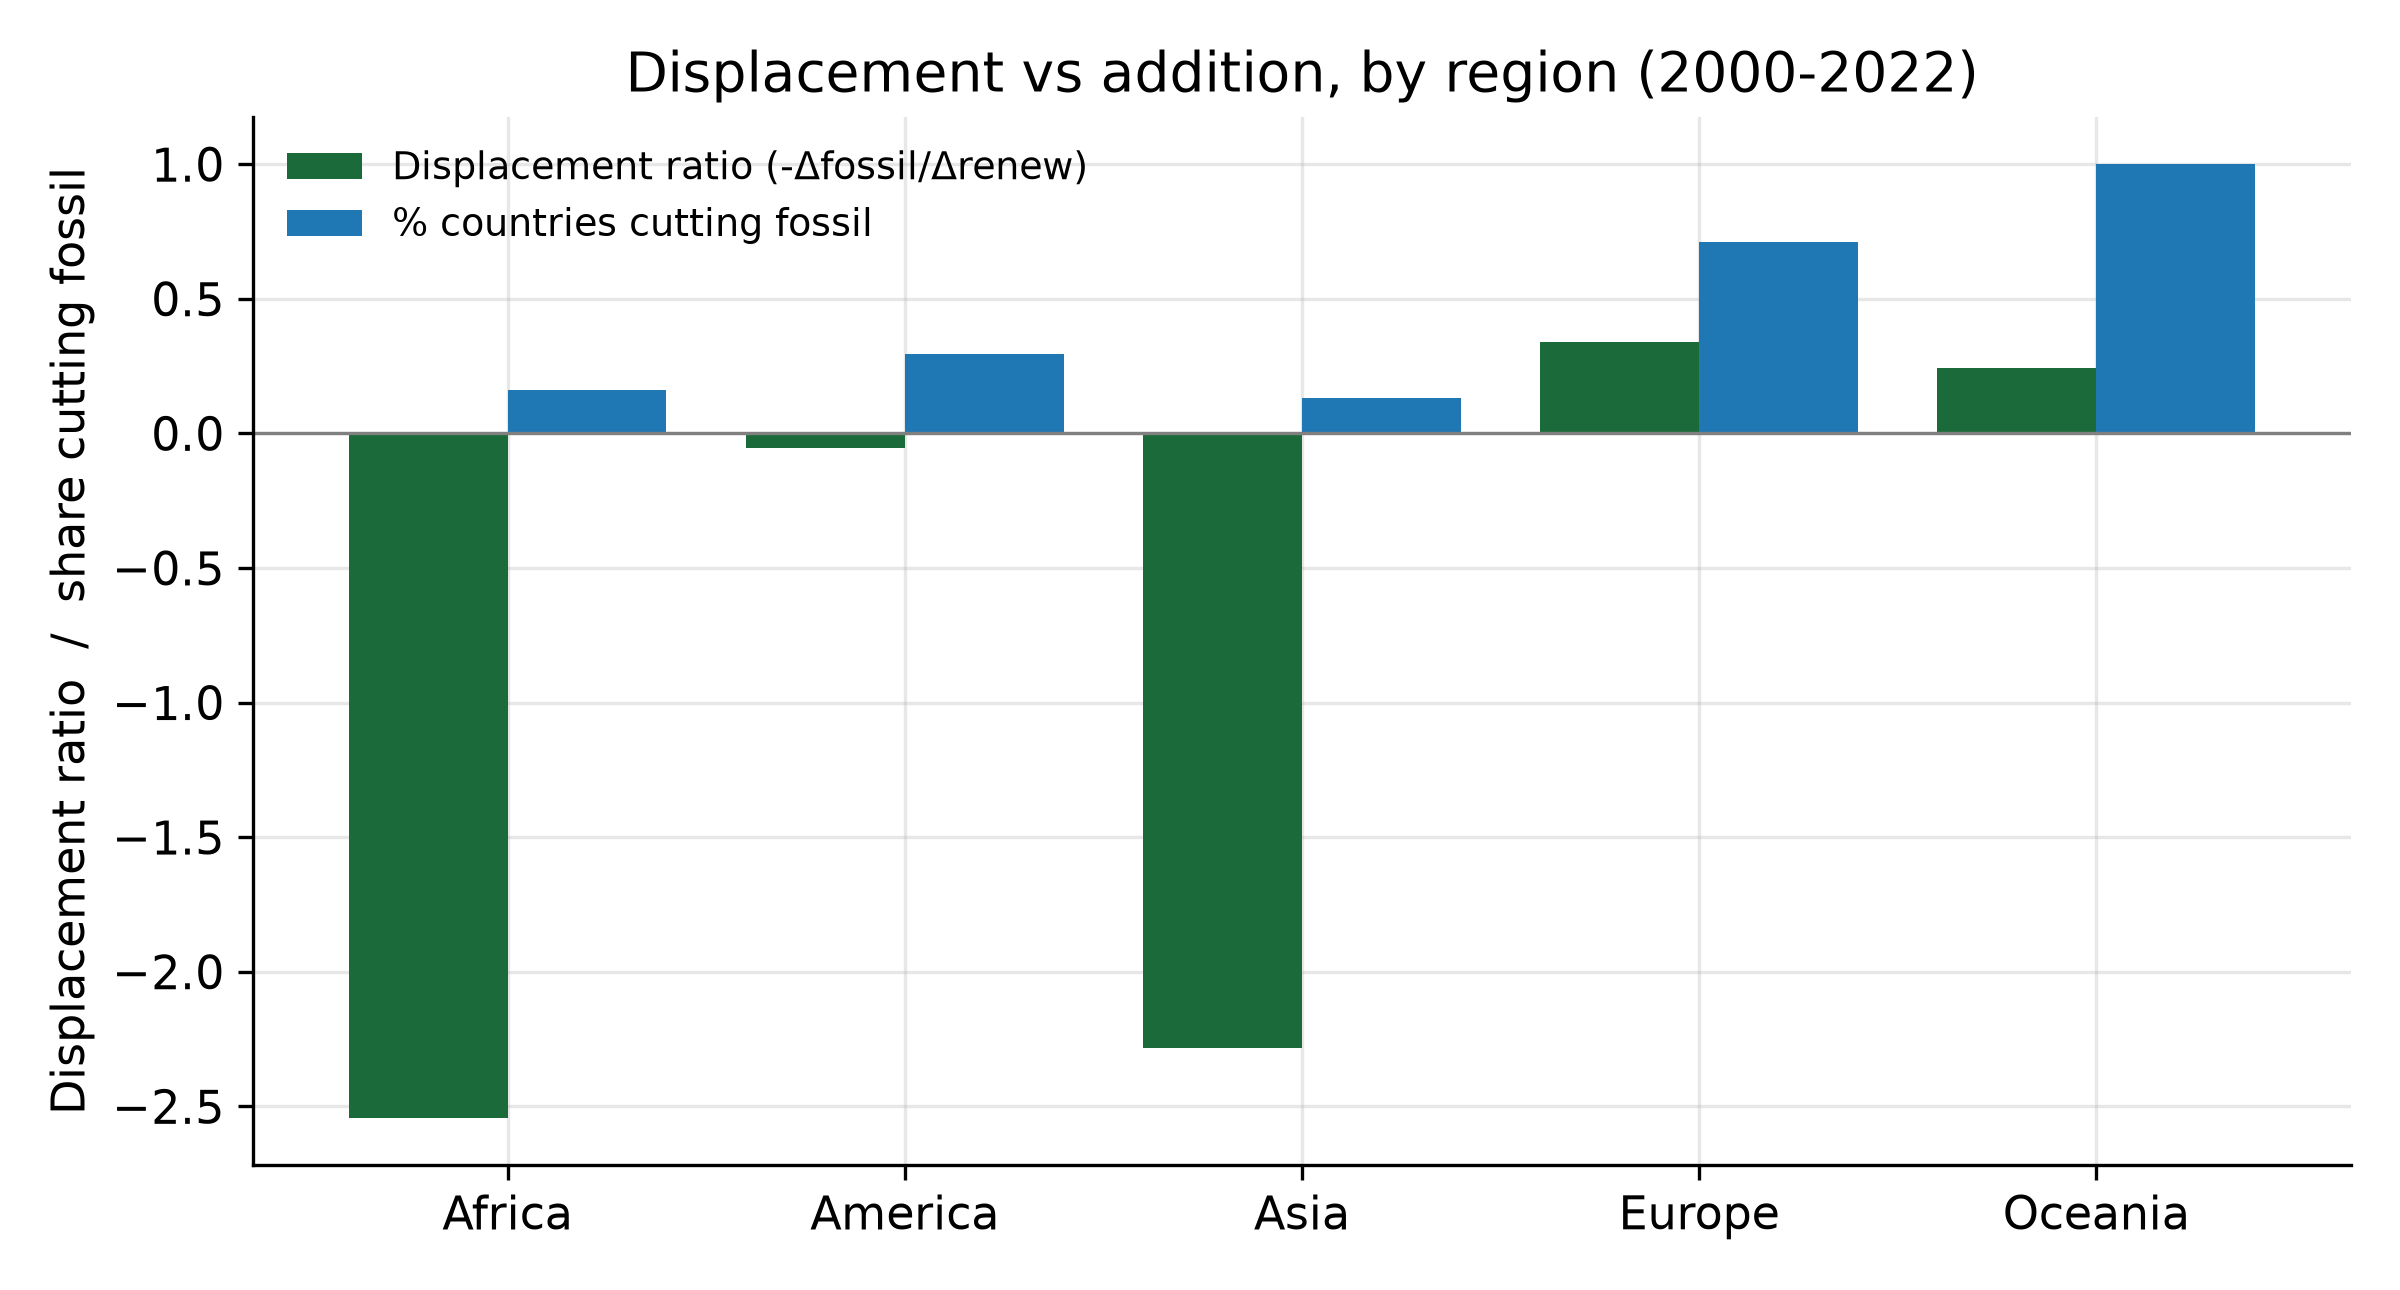
\includegraphics[width=0.8\textwidth]{figures/figure11_displacement_regional.png}
\caption{Displacement vs addition by region. Europe displaces; Africa and Asia add fossil far faster than renewables.}
\label{fig:dispreg}
\end{figure}

\subsection{Where this lands by 2030}
Extrapolating the last decade's momentum (0.87 points/year since 2013), the global renewable share reaches about 36\% by 2030 (95\% interval 35--37\%). The slower full-period trend gives 31\%. Either way, renewables remain well short of fossil's $\sim$61\% share.

\begin{figure}[H]
\centering
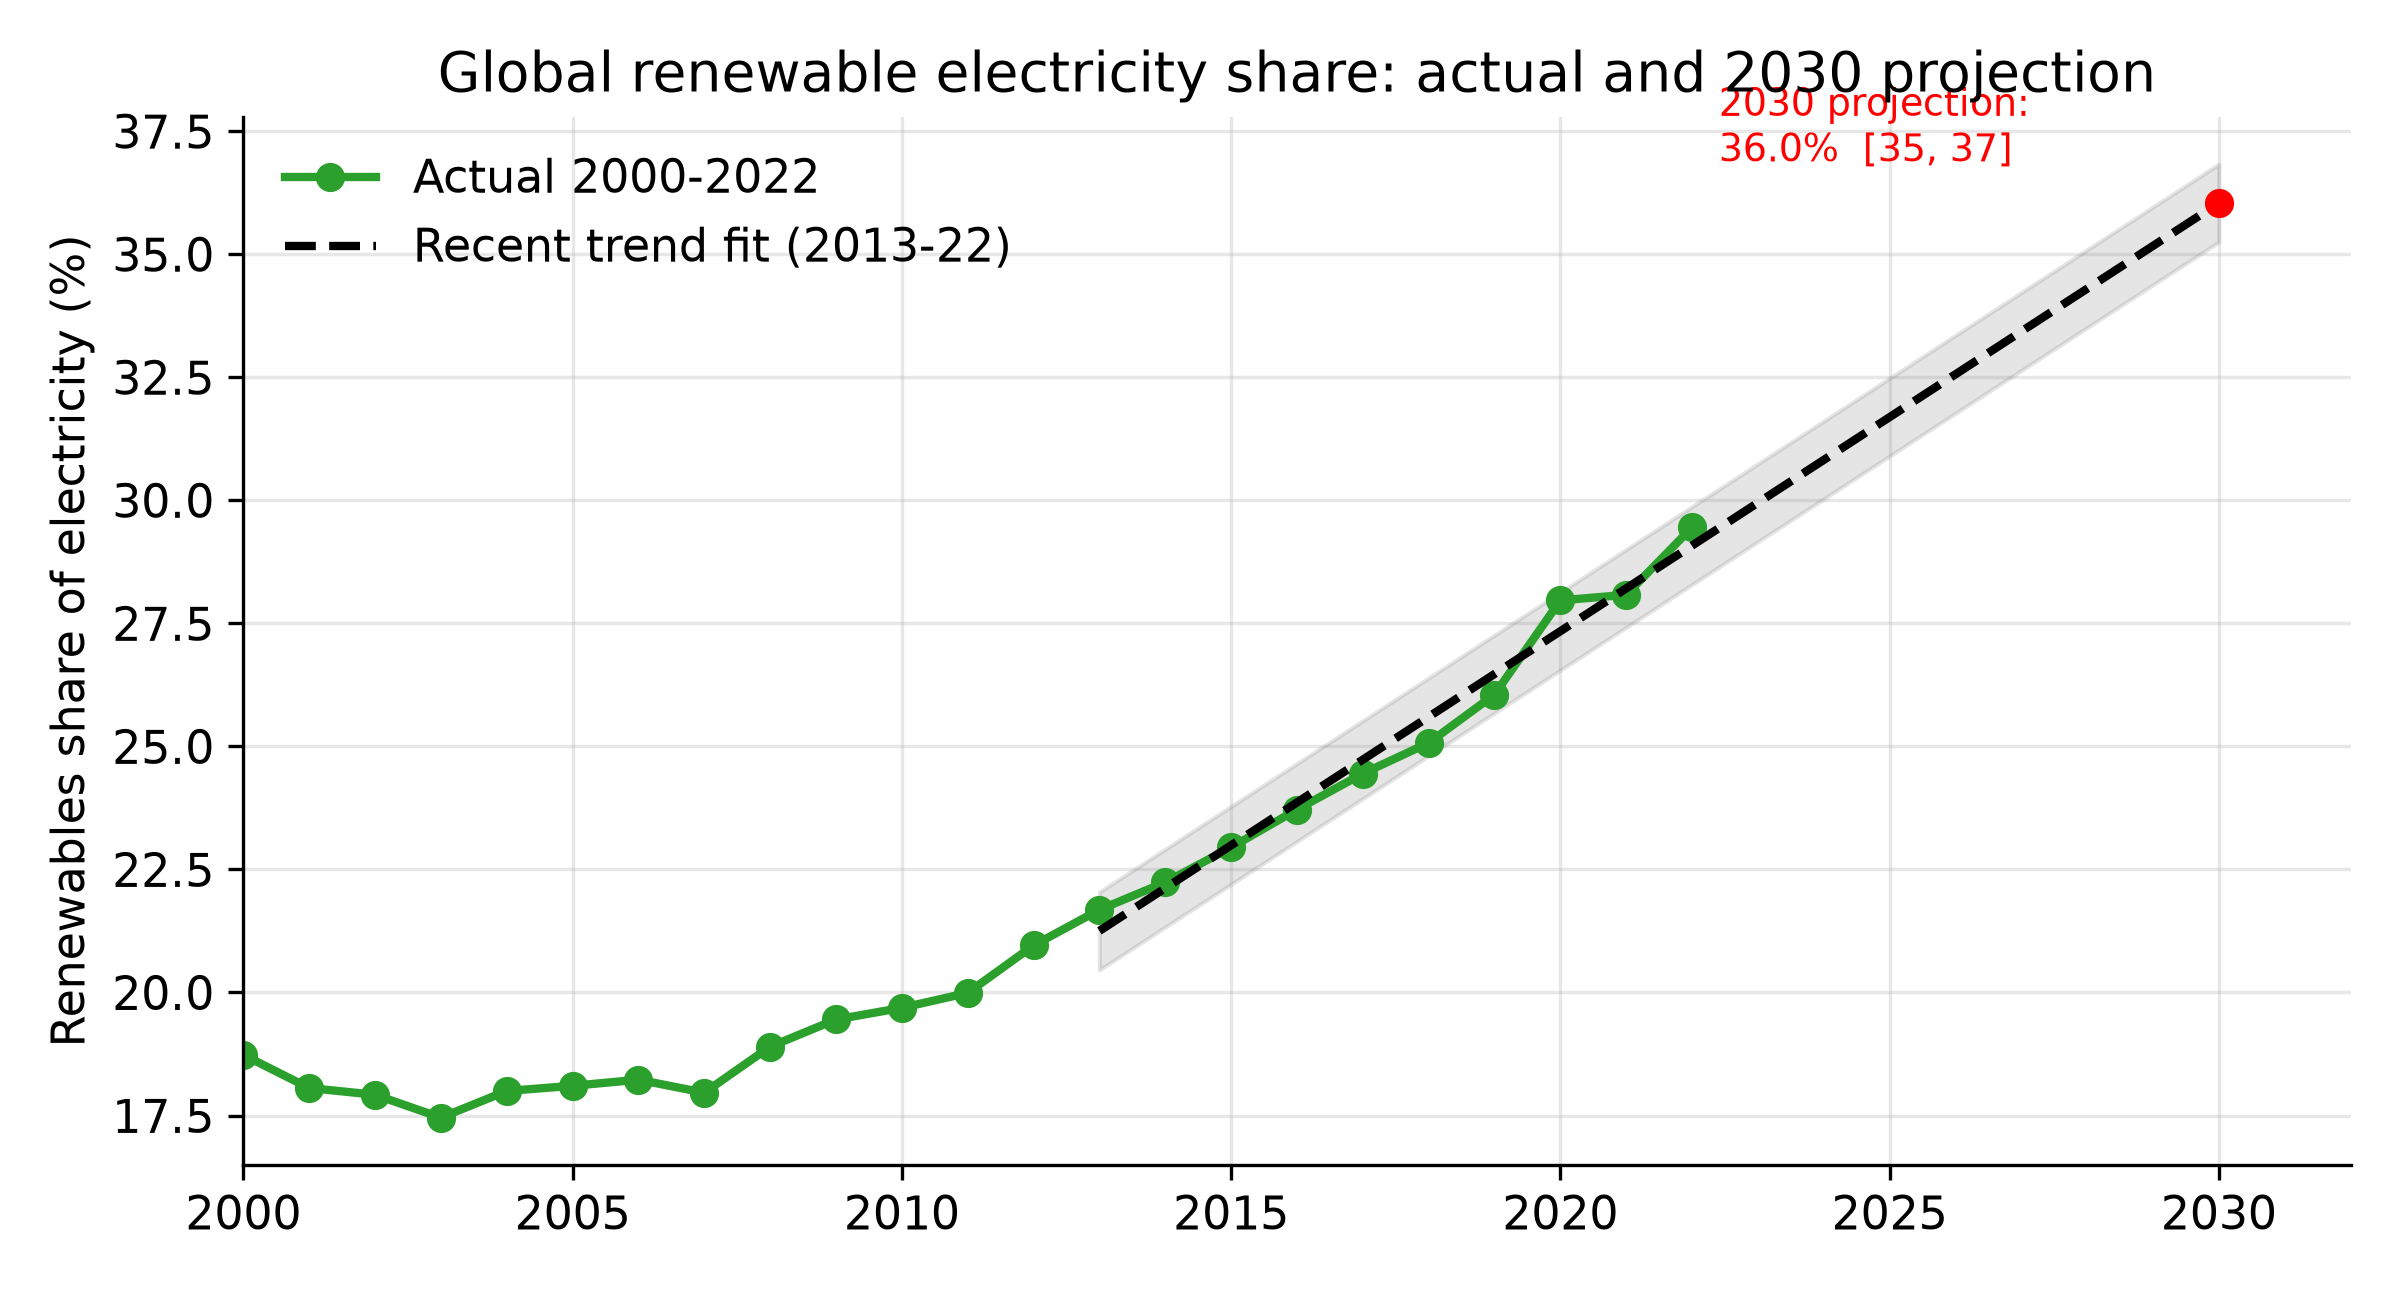
\includegraphics[width=0.8\textwidth]{figures/figure8_projection.png}
\caption{Actual renewable share and constant-momentum projection to 2030. Even on current momentum, renewables remain far below fossil's share.}
\label{fig:proj}
\end{figure}

\section{Robustness}
The baseline result survives a battery of challenges (Table~\ref{tab:rob}). Restricting to 2010--2022 leaves the coefficient at $-0.50$/pp; dropping the top-5\% emitting countries gives $-0.40$/pp; and clustering standard errors by country barely moves the inference. None of these perturbations reverses the sign or the significance of the renewable--emissions link.

\begin{table}[H]
\centering
\caption{Robustness of the renewable--emissions coefficient (country + year FE). Coef is the change in $\ln(\text{CO}_2\text{ pc})$ per $+1$ pp renewable share. *** $p<0.01$.}
\label{tab:rob}
\begin{tabular}{lccc}
\toprule
Specification & Coef & SE & N \\
\midrule
Baseline (Country + Year FE) & $-0.00607^{***}$ & 0.00057 & 3,749 \\
Sub-sample 2010--2022 & $-0.00858^{***}$ & 0.00086 & 2,119 \\
Drop top-5\% emitters & $-0.00601^{***}$ & 0.00060 & 3,565 \\
Cluster-robust SE (baseline) & -- & 0.00200 & 3,749 \\
\bottomrule
\end{tabular}
\end{table}

\section{Discussion}
The evidence points one way on pace and another on chemistry. The transition is accelerating and converging -- this is not a few leaders pulling away. Decoupling is becoming more common and more absolute, so the link between growth and carbon is weakening in practice, not only on paper. And the renewable--emissions link holds under fixed effects, lagging, first-differencing, clustered errors and a direct grid-intensity test.

But the mechanism section draws a harder line. Renewables are lowering emissions \emph{per unit of output} in most of the world, yet fossil generation keeps rising in absolute terms -- globally by more than renewables rose. The countries where the fixed-effects coefficient is strongest, Europe above all, are also the ones that retired or throttled carbon plant as they built clean capacity. Africa and Asia show no such dividend because their clean build runs alongside, not against, fossil expansion. The lesson is not that renewables fail; it is that decarbonization follows from \emph{displacement}, and displacement has to be engineered into the build, not assumed from the share.

The remaining gap is the one that matters most. Electricity is roughly half of final energy; transport, heat and industry are harder to clean, and they are where the fossil terawatt-hours really live. A 36\% renewable electricity share by 2030 is real progress and still leaves fossil dominant in power, and more so in energy overall. We are decoupling GDP from power-sector CO\textsubscript{2}. We have barely started on total emissions.

\section{Limitations}
The analysis is associational. Fixed effects, lagging, clustering and first-differencing strengthen the claim but cannot rule out all confounding -- for example, a country that decarbonizes for unrelated policy reasons may also invest in renewables, and the model would attribute the emissions fall to the renewable share. The data are secondary aggregates from OWID; country coverage and methodology revisions can shift country-year values, though the broad patterns here are robust to the standard OWID processing. Electricity-embedded emissions ignore traded-goods carbon leakage, so absolute decoupling in one country may partly reflect offshored production. The grid carbon-intensity result is the cleanest mechanism test but still cannot separate retirement of fossil plant from a shift in the dispatch order without unit-level data. The 2030 projection is a constant-momentum extrapolation, not a scenario with policy or price responses, and should be read as a floor under current behaviour rather than a forecast.

\section{Conclusion}
The renewable electricity transition is real, it is accelerating, and in most of the world it is decoupling growth from CO\textsubscript{2} emissions. The countries that started furthest behind are catching up fastest, and absolute decoupling is spreading. The catch is in the arithmetic: the world added renewables and added fossil at the same time, and fossil won the terawatt-hour race. Only 31\% of countries cut fossil generation at all. So the transition is genuine and yet, in the aggregate, still additive.

That single fact reframes the policy question. The goal is not to build clean power faster than demand grows -- the record shows that, by itself, does not retire carbon. The goal is to retire carbon. Every mechanism in this paper points to the same lever: make renewables displace, not accompany. Do that, and the decoupling already visible in Europe becomes the global default instead of the exception.

\section*{Data and code availability}
Data are from Our World in Data's energy and CO\textsubscript{2} datasets (CC-BY; ourworldindata.org/energy-data), used under the Open Data Commons Attribution License. The complete analysis pipeline, figures, and this manuscript are reproducible from the scripts in the project repository: \texttt{src/analysis.py} computes every statistic and figure from the raw CSVs into \texttt{results.json}; \texttt{src/build\_report.py} and \texttt{src/build\_dashboard.py} render the HTML report and the interactive dashboard. Re-running \texttt{python src/analysis.py} regenerates all numerical results. No restricted or proprietary data were used.

\begin{thebibliography}{12}
\bibitem[Tapio(2005)]{tapio} Tapio, P. (2005). Towards a theory of decoupling: degrees of decoupling in the EU and the case of road traffic vs GDP, 1970--2001. \emph{Transport Policy}, 12(2), 137--151.
\bibitem[OECD(2002)]{oecd} OECD (2002). \emph{Indicators to measure decoupling of environmental pressure from economic growth}. OECD, Paris.
\bibitem[Steinberger \& Roberts(2010)]{steinberger} Steinberger, J. K. \& Roberts, J. T. (2010). From constraint to sufficiency: the decoupling of energy and carbon from human needs. \emph{Environmental Research Letters}, 5(3), 034019.
\bibitem[Jackson \& Papathanasopoulou(2008)]{jackson} Jackson, T. \& Papathanasopoulou, E. (2008). Luxury or `lock-in'? An exploration of unsustainable consumption in the UK. \emph{Ecological Economics}, 68(1--2), 80--95.
\bibitem[Semieniuk et al.(2021)]{semieniuk} Semieniuk, G., Campiglio, E. \& Mercure, J. F. (2021). Low-carbon transition, green growth and the macroeconomic consensus. \emph{Ecological Economics}, 179, 106832.
\bibitem[IPCC(2022)]{ipcc} IPCC (2022). \emph{Climate Change 2022: Mitigation of Climate Change}. Cambridge University Press.
\bibitem[IEA(2023)]{iea} IEA (2023). \emph{World Energy Outlook 2023}. OECD/IEA.
\bibitem[Hickel \& Kallis(2020)]{hickel} Hickel, J. \& Kallis, G. (2020). Is Green Growth Possible? \emph{New Political Economy}, 25(4), 469--486.
\bibitem[Poumanyvong \& Kaneko(2010)]{poumanyvong} Poumanyvong, P. \& Kaneko, S. (2010). Does urbanization lead to less energy use and lower CO\textsubscript{2} emissions? \emph{Ecological Economics}, 70(2), 434--444.
\bibitem[Ritchie et al.(2024)]{owid} Ritchie, H., Roser, M. \& Rosado, P. (2024). \emph{CO\textsubscript{2} and Greenhouse Gas Emissions}. Our World in Data.
\bibitem[Brockway et al.(2019)]{brockway} Brockway, P. E., Heun, M. K., Santos, J. \& Barrett, J. R. (2019). Energy rebound, economy-wide impacts and the global economy. \emph{Energy}, 174, 258--267.
\bibitem[Our World in Data(nd)]{owid-data} Our World in Data. \emph{Energy and CO\textsubscript{2} datasets} (CC-BY). ourworldindata.org/energy-data
\end{thebibliography}

\end{document}
